\Chapter{IBD Prompt Energy Spectrum of Antineutrinos from $^{235}$U}
\label{Ch9}

With event selections based on multiple aspects of the prompt and delayed coincidence and cosmic ray exclusion, PROSPECT is able to detect reactor neutrinos with minimal overburden.
The first reactor neutrino oscillation measurement from PROSPECT~\cite{bib:prospect_osc} was made using 33 exposure days reactor-on and 30 exposure days of reactor-off data. 
The first IBD prompt energy spectrum of antineutrinos from HFIR was measured after $\sim$78 days (40.3 reactor-on exposure days, 37.8 reactor-off exposure days) of total data acquisition~\cite{bib:prospect_spec}.
In this thesis, the IBD prompt energy spectrum measurement is reported.
Because of the limited detector dynamic range and the energy range of IBD prompt energy, the prompt energy spectrum between 0.8~MeV and 7.2~MeV is studied. 
The reactor correlated energy spectrum is obtained with reactor off backgrounds subtracted from reactor on IBD candidates.
To do this, delicate background stability characterization and corrections were performed.
To quantify the contribution of $^{235}$U to the 5-7~MeV excess of the reactor neutrino spectrum with respect to the Huber model~\cite{bib:huber}, the PROSPECT measured IBD spectrum was compared to a variety of spectrum models. 

\Section{IBD Event Selection}

The reconstructed IBD event rate and energy spectrum was blinded until the IBD event selection values were frozen.
PROSPECT's initial reactor neutrino oscillation measurement was based on IBD event selection developed with 3~days of reactor-on and reactor-off data.
The IBD selection for the prompt energy spectrum measurement was further studied with the oscillation measurement data before unblinding additional data. 
Some IBD selection values were adjusted to optimize signal stability, signal to background ratio (S:B), and total event statistics.

The IBD event selections are selections based on PSD, time coincidence between prompt and delayed clusters, topological spread of the IBD clusters, and detector volume cuts.
Acceptance values of IBD selection and the physical purpose of each cut are shown in Table~\ref{tab:IBDcuts}.
The PSD values of prompt and delayed hits are used to identify the type of particle.

%\begin{table}

    \begin{longtable}{p{3cm}p{2.5cm}p{4cm}p{4cm}}    
    %\center
    \caption[IBD event selection]{All cuts of IBD event selections.}\\
    \hline
    \hline
    Event Class  & Category   & Accepted value  & Purpose  \\ 
    \hline
    Prompt  & PSD  & $< 2.5 \sigma$ of lower PSD distribution & Purify positron and gamma selection  \\
    \hline
    $n$-Li  & PSD  & $< 3.6 \sigma$ of $n$-Li PSD distribution  & select $n$-Li hits based their PSD range \\
        & energy  & $< 3 \sigma$ of $n$-Li energy distribution  & select $n$-Li hits based energy range  \\
    \hline
    Prompt-delay correlations     &  $\Delta t$    &  1-120 \textmu s & maximize the window for the delayed $n$-Li hits \\
    		& $\Delta (x, y)$ & same segment or adjacent segment (0 to 14.5~cm) & close prompt-delay vertex\\
    		& $\Delta z$ & 180~mm (same segment) 140~mm (adjacent segment) &  close prompt-delay vertex\\
    \hline
     Cosmic shower   & muon veto & $>|200|$~\textmu s from a muon event  & reject accidental background correlated with muon shower  \\
       & fast neutron veto  &  $>|200|$~\textmu s from a uncorrelated $n$-Li hit &  reject accidentals correlated with cosmic neutron  \\
       & heavy particle recoil veto  &  $>|200|$~\textmu s from a uncorrelated from heavy particle & reject accidentals correlated with cosmic shower  \\
    \hline
    Fiducial volume  & $z$ range & $<$44.4~cm from segment center  & veto accidentals with the scintillator at edges  \\
        & segment exclusion & prompt vertex inside the fiducial volume &  veto accidentals with the scintillator at edges \\
    \hline
     \label{tab:IBDcuts}
     \end{longtable}

%\end{table}

In the study of optimizing IBD selection, an \textit{effective count} was defined as 
\begin{equation}
	\mathrm{Effective count} = \sum_{0.8\mathrm{MeV}}^{7.2\mathrm{MeV}}\frac{1}{\sigma^2_{relative}},
\end{equation}
where
\begin{equation}
 \sigma_{relative} = \sqrt{\sigma_{on}^2 + \sigma_{off}^2+2(5\%*\sigma^2_{off})}.
\end{equation}
Both $\sigma_{on}$ and $\sigma_{off}$ consist of a statistical uncertainty and 5\% systematic uncertainty of IBD candidates collected in the reactor-on and -off period, respectively.
Additionally, the reactor off normalization uncertainty of 5\% of the total uncertainty was added under the consideration of the time dependence of the IBD rate. 
The IBD selection was optimized by searching for various acceptance values to maximize the effective count.

The PSD selection of prompt and delayed hits are based on the PSD distribution of all events collected in a one~hour run.
The PSD distribution of all hits in the PROSPECT detector, as well as an illustration of the IBD coincident hit selection are shown in Figure~\ref{fig:IBDPSD}.
By selecting events dynamically with PSD distributions, the time dependence of particle identification is minimized.
\begin{figure}[h!]
    \centering
    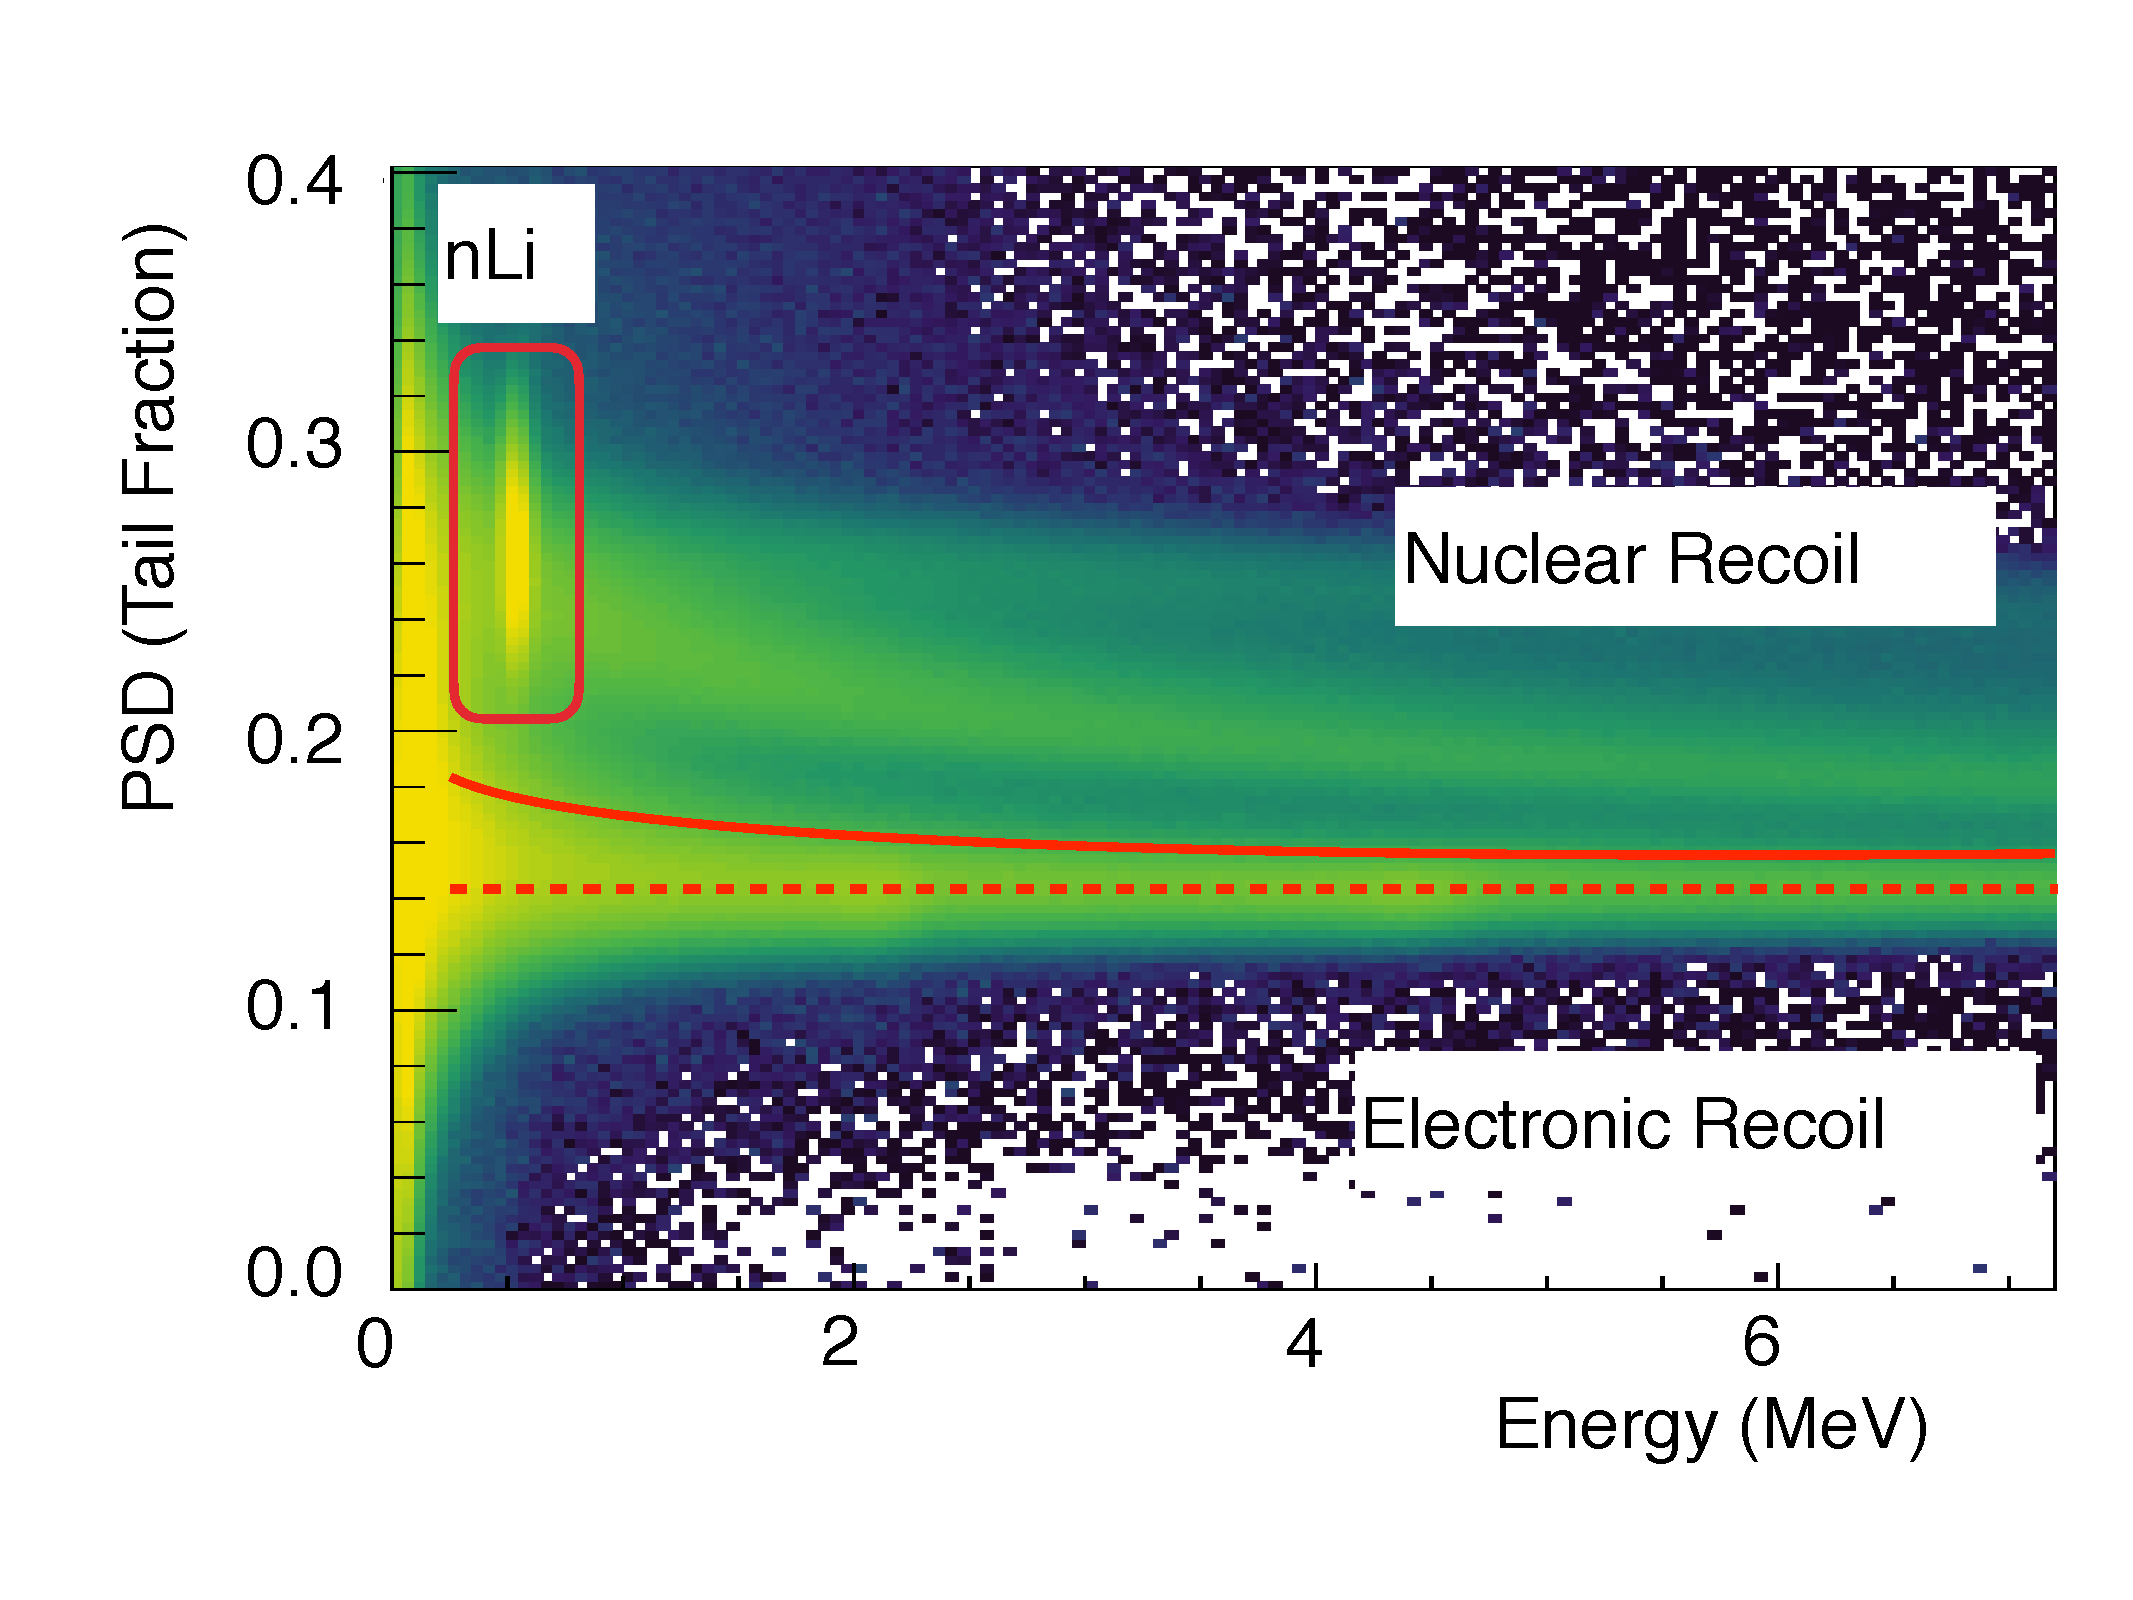
\includegraphics[width=0.6\textwidth]{Figures/IBDPSD.pdf}
    \caption[Illustration of IBD PSD selection]{Illustration of the IBD PSD selection, where the solid line and dashed line are 2.5$\sigma$ threshold for positron- and gamma-like hits and the mean of their PSD distribution.
    The red circle represents the small range of PSD and energy for $n$-Li-capture-like hits.}
    \label{fig:IBDPSD}
\end{figure}

The time coincidence of prompt and delayed clusters requires a 1 to 120~\textmu s $\Delta t$ window, that is 
\begin{equation}
\Delta t \equiv T_{delayed} - T_{prompt}
\end{equation}
Other time cuts are applied to minimize accidental IBD candidate (henceforth referred to as `accidental') rates, cosmogenic showers, and fast neutrons of cosmic ray backgrounds and reactor correlated non-IBD events.
Topology cuts require close distance prompt and delayed hits to further reduce accidentals. 
In the PG4 simulation of the detector response to cosmic backgrounds, the out-most layer of segment was found to contain significantly more backgrounds than the inner segments.
Thus, IBD prompt hits in the exterior segments are excluded.
The interior segments of the PROSPECT AD are referred to as the \textit{fiducial volume}.
Once again, the finalized IBD selection values are listed in Table~\ref{tab:IBDcuts}. 
The simulated IBD prompt energy spectrum is shown in Figure~\ref{fig:IBDCuts}.

\begin{figure}[h!]
    \centering
    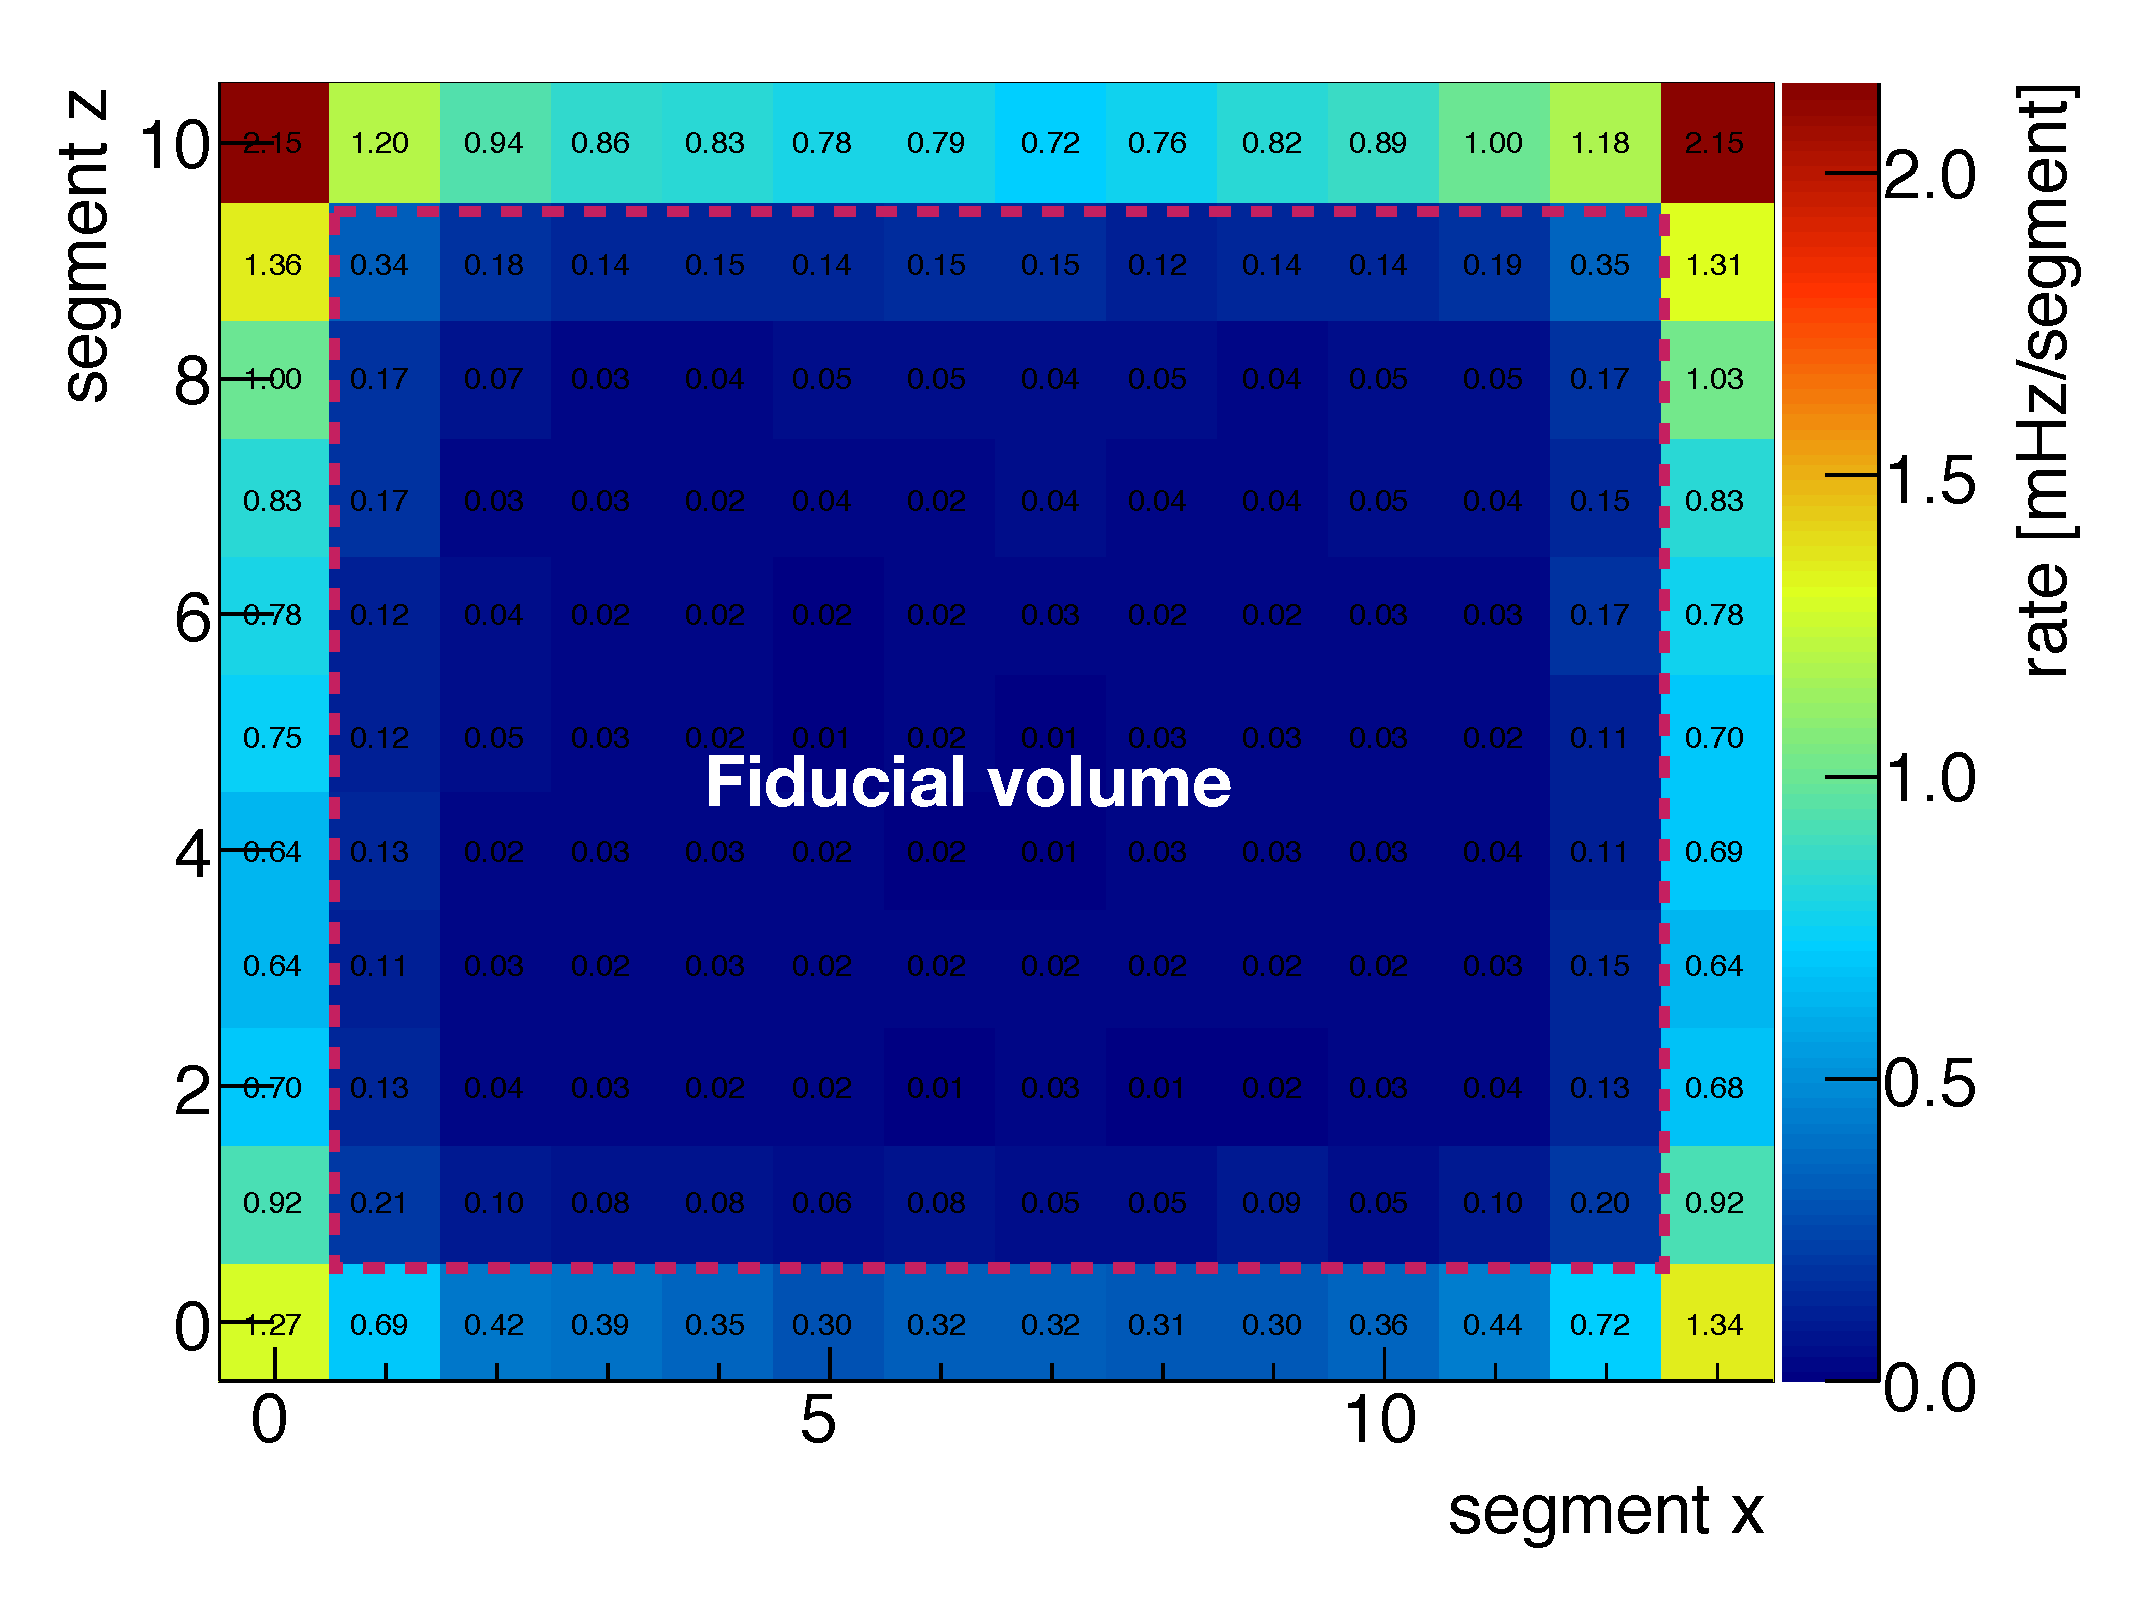
\includegraphics[width=0.6\textwidth]{Figures/Fiducial.pdf}
    \caption[Illustration of the detector fiducial volume]{Illustration of the detector fiducial volume from the PG4 simulation of the cosmic ray background, where the accidental rate of each segment is shown. 
    The higher accidental rate in the exterior segments lead to selection of IBD candidates within the fiducial volume.}
    \label{fig:Fiducial}
\end{figure}

\begin{figure}[h!]
    \centering
    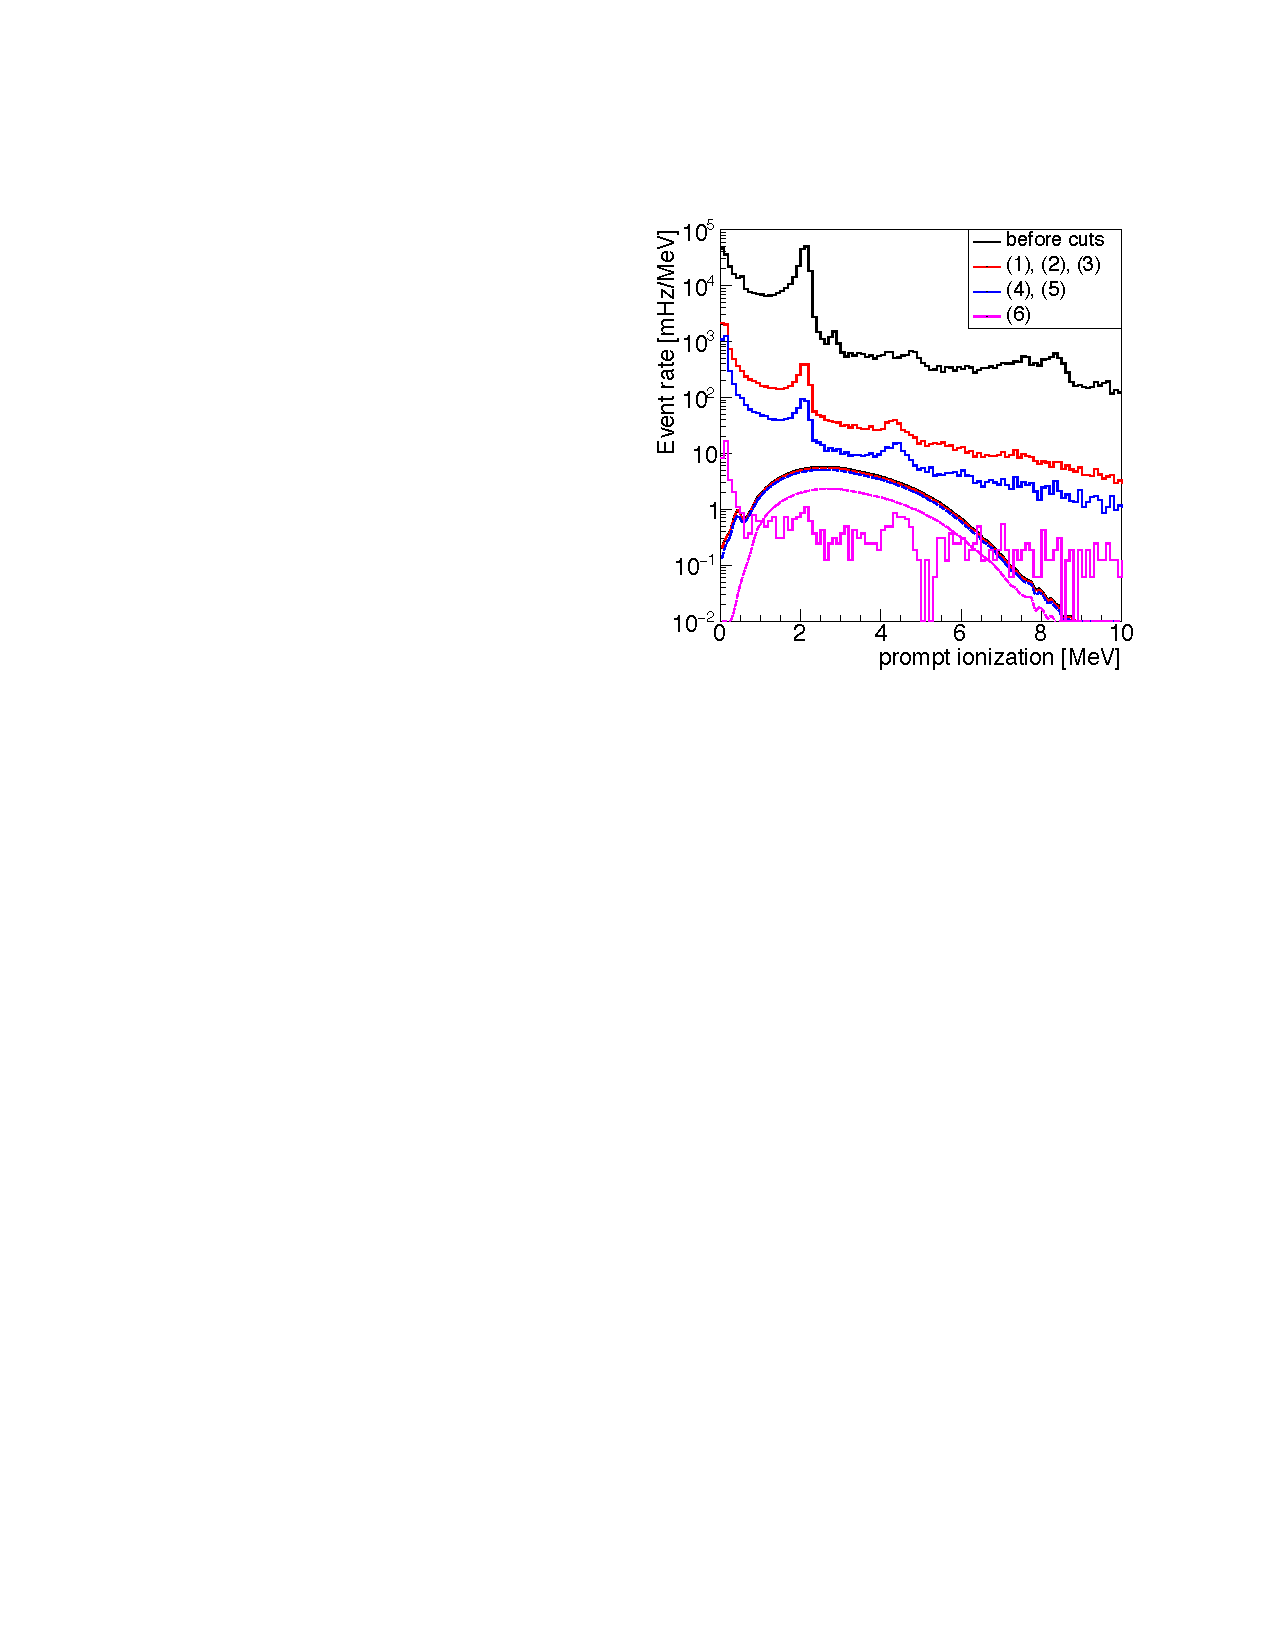
\includegraphics[width=0.6\textwidth]{Figures/IBDCuts.pdf}
    \caption[Different levels of IBD selection]{
    The amount of IBD candidates and cosmic backgrounds passing different levels of IBD selection cuts.
    (1, 2, 3) Cosmic background veto time windows, including muon veto, fast neutron, and single nuclear recoils.
    (4, 5) Topological cut of prompt and delay distance.
    (6) Fiducial volume.
    }
    \label{fig:IBDCuts}
\end{figure}

\Section{Observation of Reactor Neutrinos on Earth's Surface}

PROSPECT is able to detect reactor neutrinos with minimal overburden.
With the first two-hour reactor-on dataset, PROSPECT is able detect a $>5\sigma$ signal of reactor neutrinos from HFIR.
In the first 24 hours of reactor-on data acquisition and the same duration of reactor-off data, the PROSPECT AD collected 1254 $\pm$30 reactor on correlated IBD events and 614$\pm$20 reactor-off IBD-like candidates.
PROSPECT's capability of detecting reactor neutrinos under high cosmic backgrounds is due to the precise timing and topological cuts enabled by optical segmentation and PSD.

\begin{figure}[h!]
    \centering
    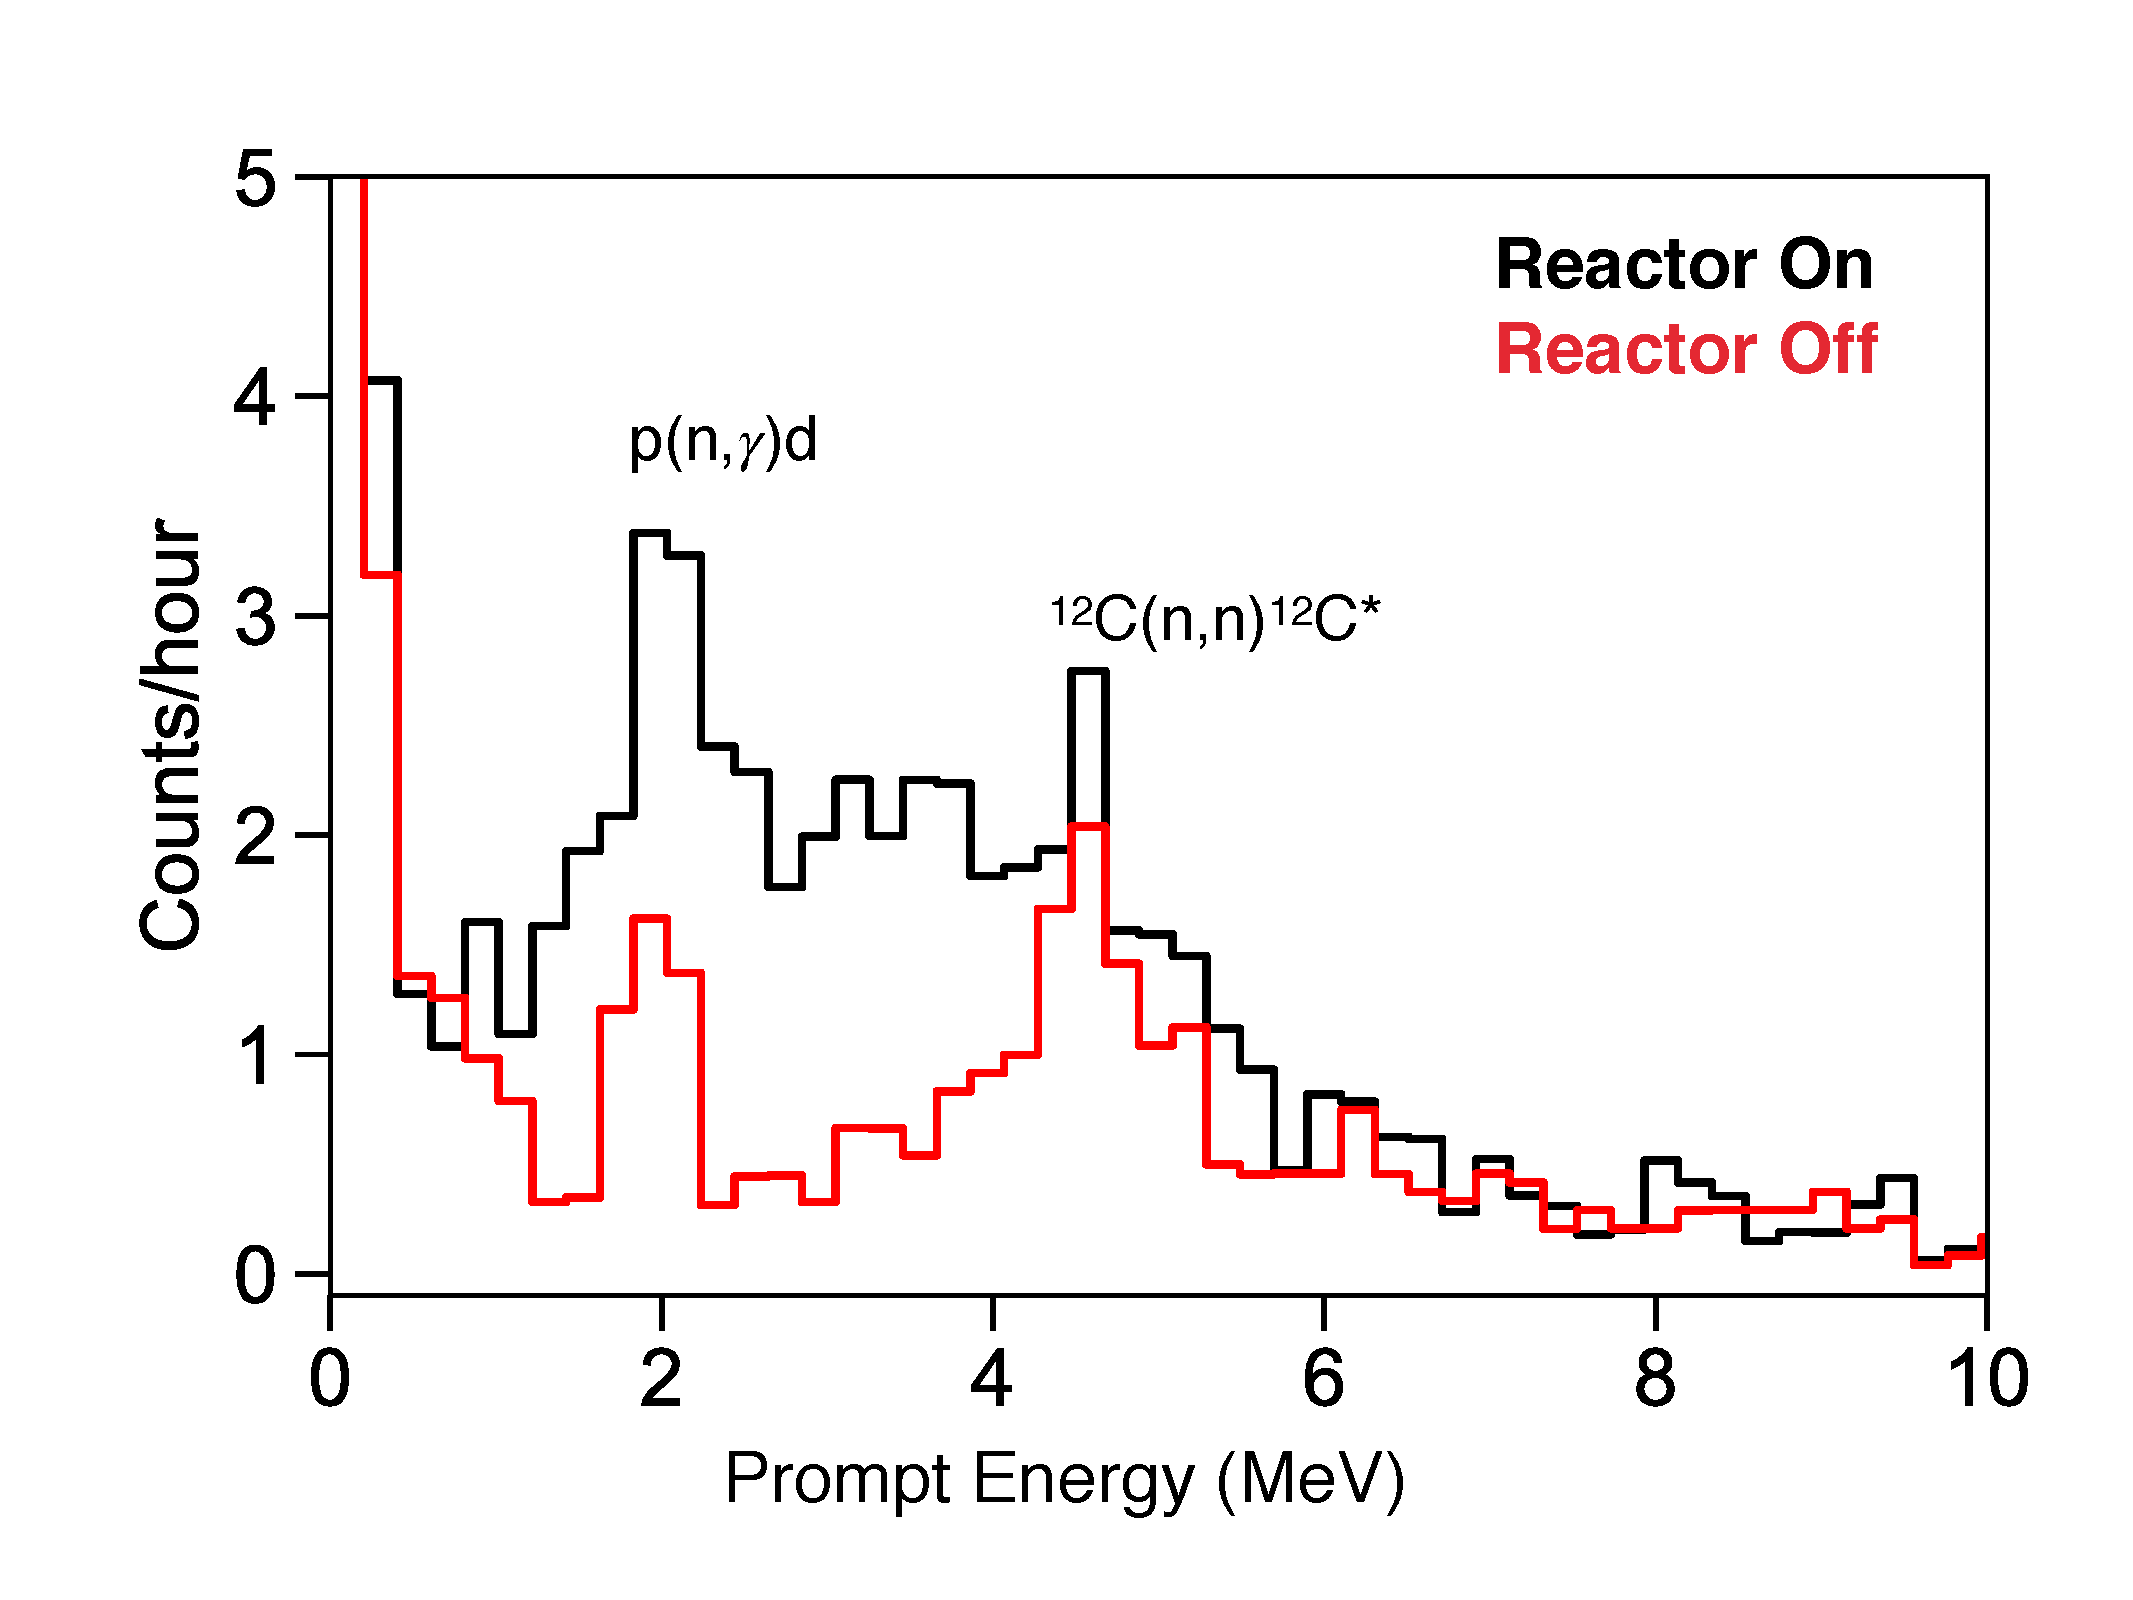
\includegraphics[width=0.6\textwidth]{Figures/FirstNeutrino.pdf}
    \caption[Reactor neutrino from HFIR]{The reactor-on and -off IBD prompt energy spectra measured with 24 hours of reactor-on and -off data, separately.
    Two major background contributions in the spectra are the cosmic IBD-like events with $n$-H capture gamma and the gamma from $n$-carbon inelastic scattering.}
    \label{fig:firstnu}
\end{figure}

\Section{Background Subtraction}

Among the selected IBD candidates, the cosmogenic neutrons are the main source of background in PROSPECT's IBD measurement.
The background mainly contains the inelastic recoil of fast neutrons, a 2.2~MeV $n$-H capture de-excitation gamma and the 4.4~MeV de-excitation gamma from $n$ carbon inelastic scattering (nC*).
Measured the IBD prompt energy spectrum is a result of background subtraction,
\begin{equation}
S_{IBD} =(S_{on-corr} - \frac{T_{corr}}{T_{acc}}S_{on-acc}) - k\cdot  \frac{T_{on}}{T_{off}} (S_{off-corr} - \frac{T_{corr}}{T_{acc}}S_{off-acc}),
\end{equation} 
where $S_{on-corr}$ ($S_{off-corr}$) is the reactor-on (-off) correlated prompt spectrum, when $1 < \Delta t < 120~$~\textmu s .
The accidental candidates are uncorrelated beta/gamma and $n$-Li capture hits defined as $-12 < \Delta t < -2$~ms in PROSPECT data analysis.
Prior to subtraction, the accidental spectrum was normalized based on the time window length with respect to the IBD coincident window.
Additionally, $k$ is a factor that varies with time that is applied to the reactor-on and reactor-off ratio to correct time dependent event rate differences.

The event rate of cosmic ray backgrounds is time dependent because of environmental atmospheric thickness variation (directly reflected by the variation of atmospheric pressure).
By comparing fast neutron, single $n$-Li capture, and muon rates to the atmospheric pressure with respect of time, the correlation between atmospheric pressure and event rates was found.
In analysis, these correlations are simplified with a linear function fitted to event rate vs. atmospheric pressure data points shown in Figure~\ref{fig:atmosphere}.
A correction factor based on atmospheric pressure was applied to the normalization of reactor-on and -off prompt energy spectra in order to subtract background correctly.
After adjustments based on atmospheric pressure, the IBD correlated candidate rates during the data acquisition period are stable, as shown in Figure~\ref{fig:IBDstability}. 

\begin{figure}[h!]
    \centering
    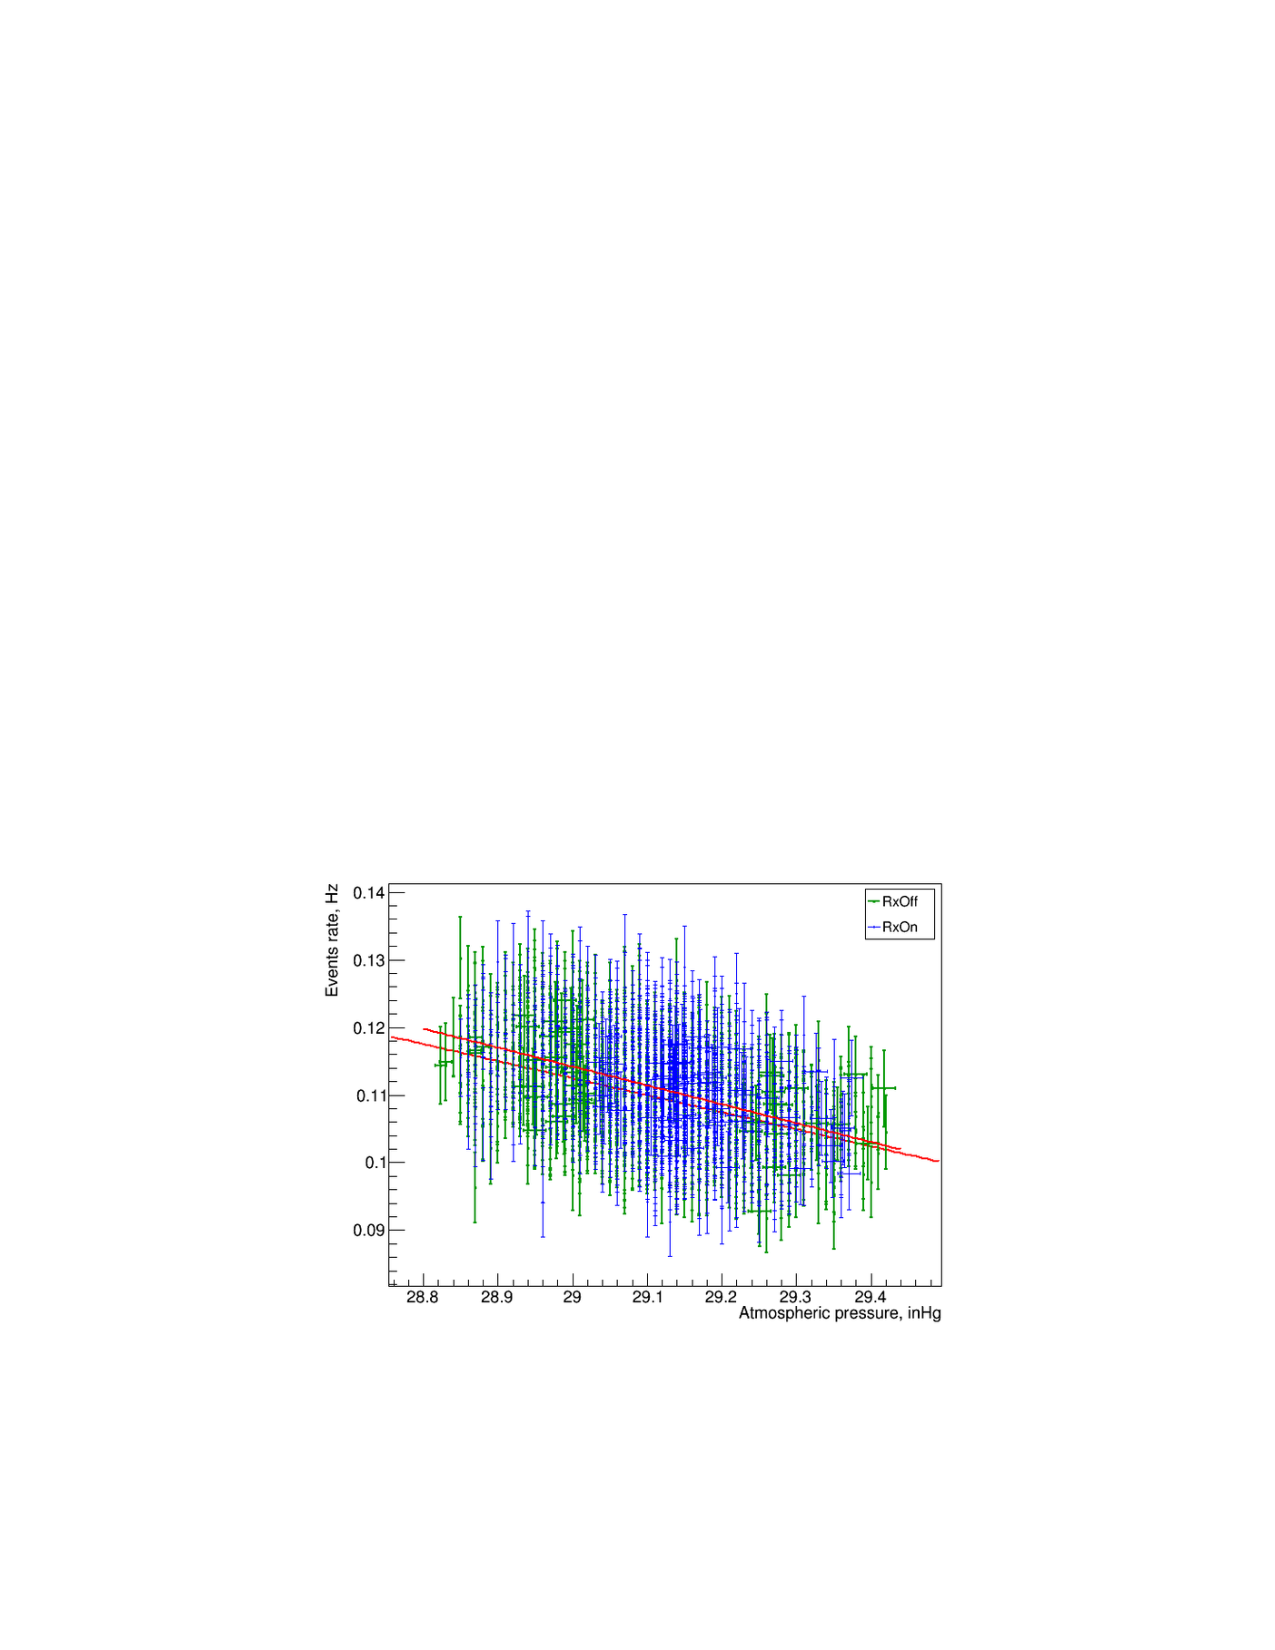
\includegraphics[width=0.7\textwidth]{Figures/FNAtmosphere.pdf}\\
    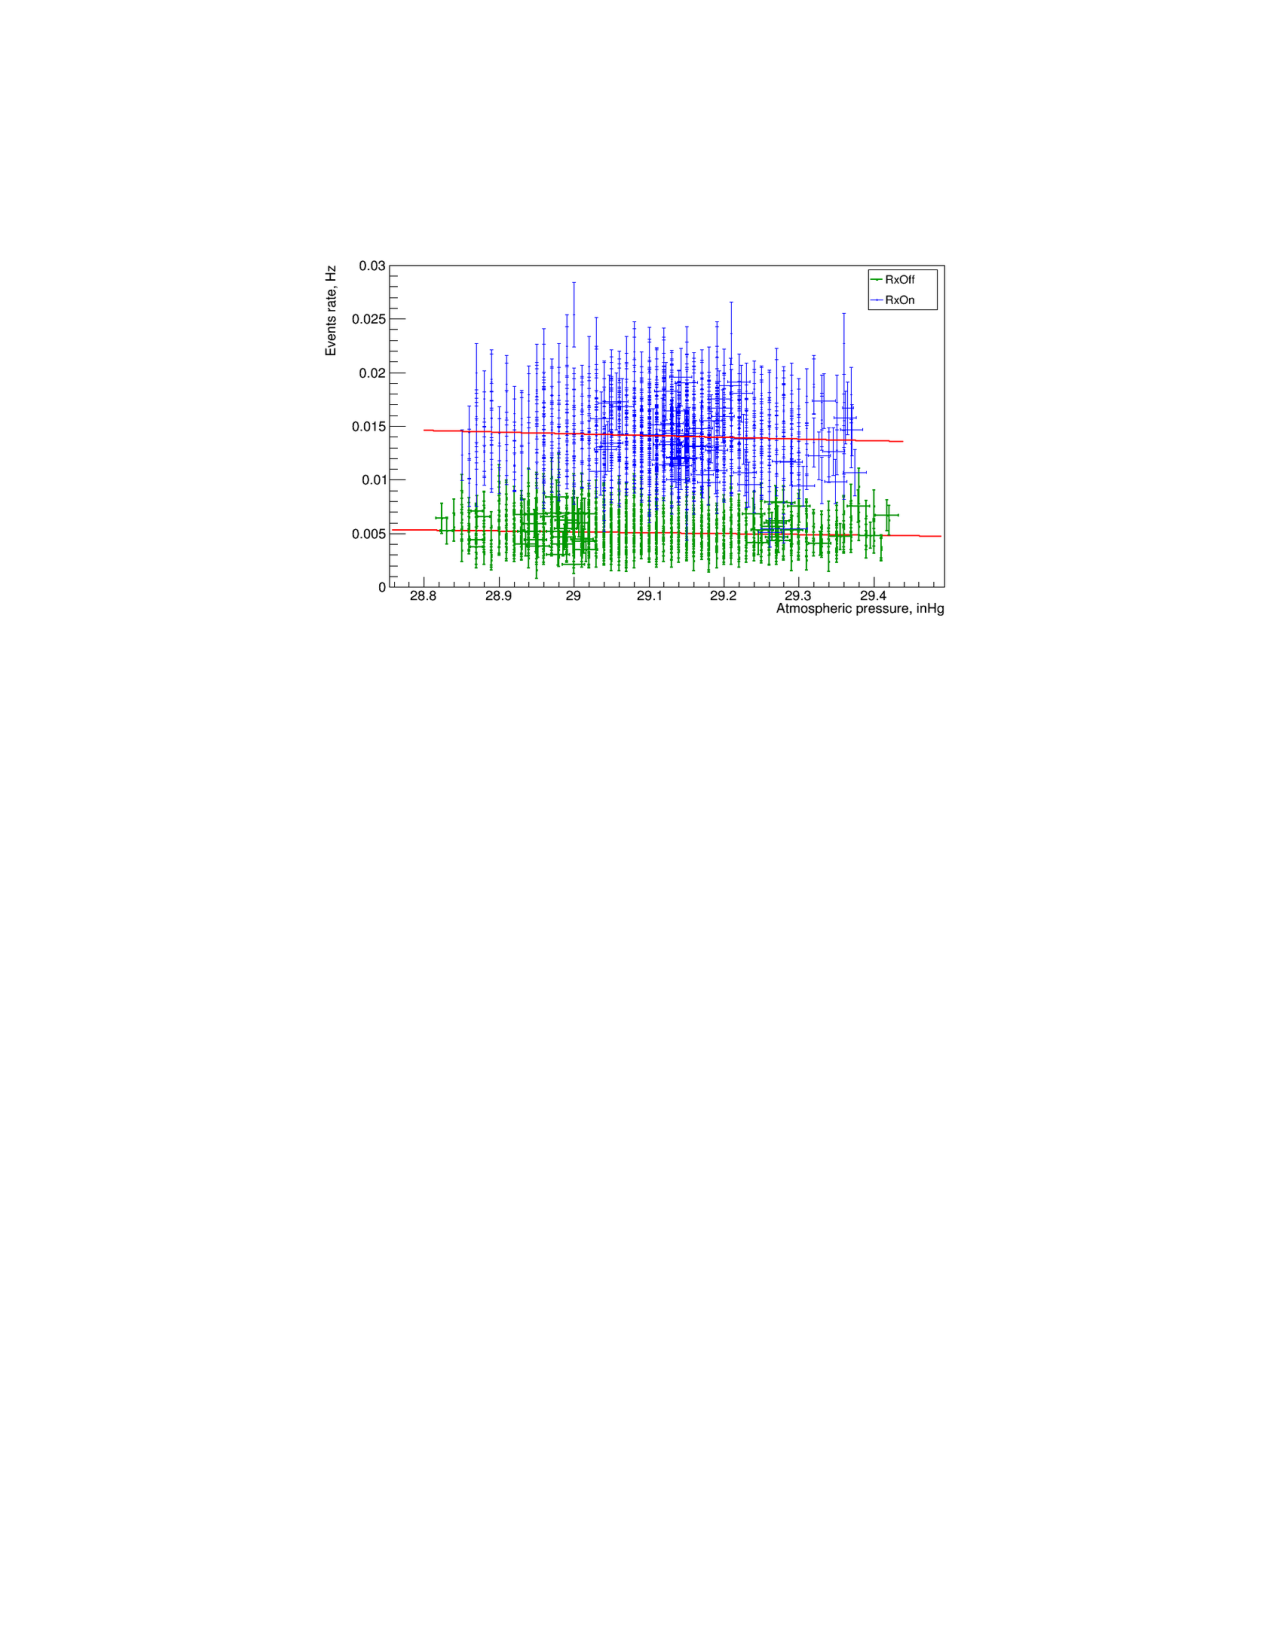
\includegraphics[width=0.7\textwidth]{Figures/IBDAtmosphere.pdf}
    \caption[Correlations between atmospheric pressure and neutron/IBD event rate.]{
    (Top) The correlation between fast neutron + single $n$-Li events and atmospheric pressure.
    (Bottom) The correlation between IBD event rate and atmospheric pressure.
    Because reactor correlated event rate is higher, the reactor-on and -off data points are fitted separately with linear functions.}
    \label{fig:atmosphere}
\end{figure}

\begin{figure}[h!]
    \centering
    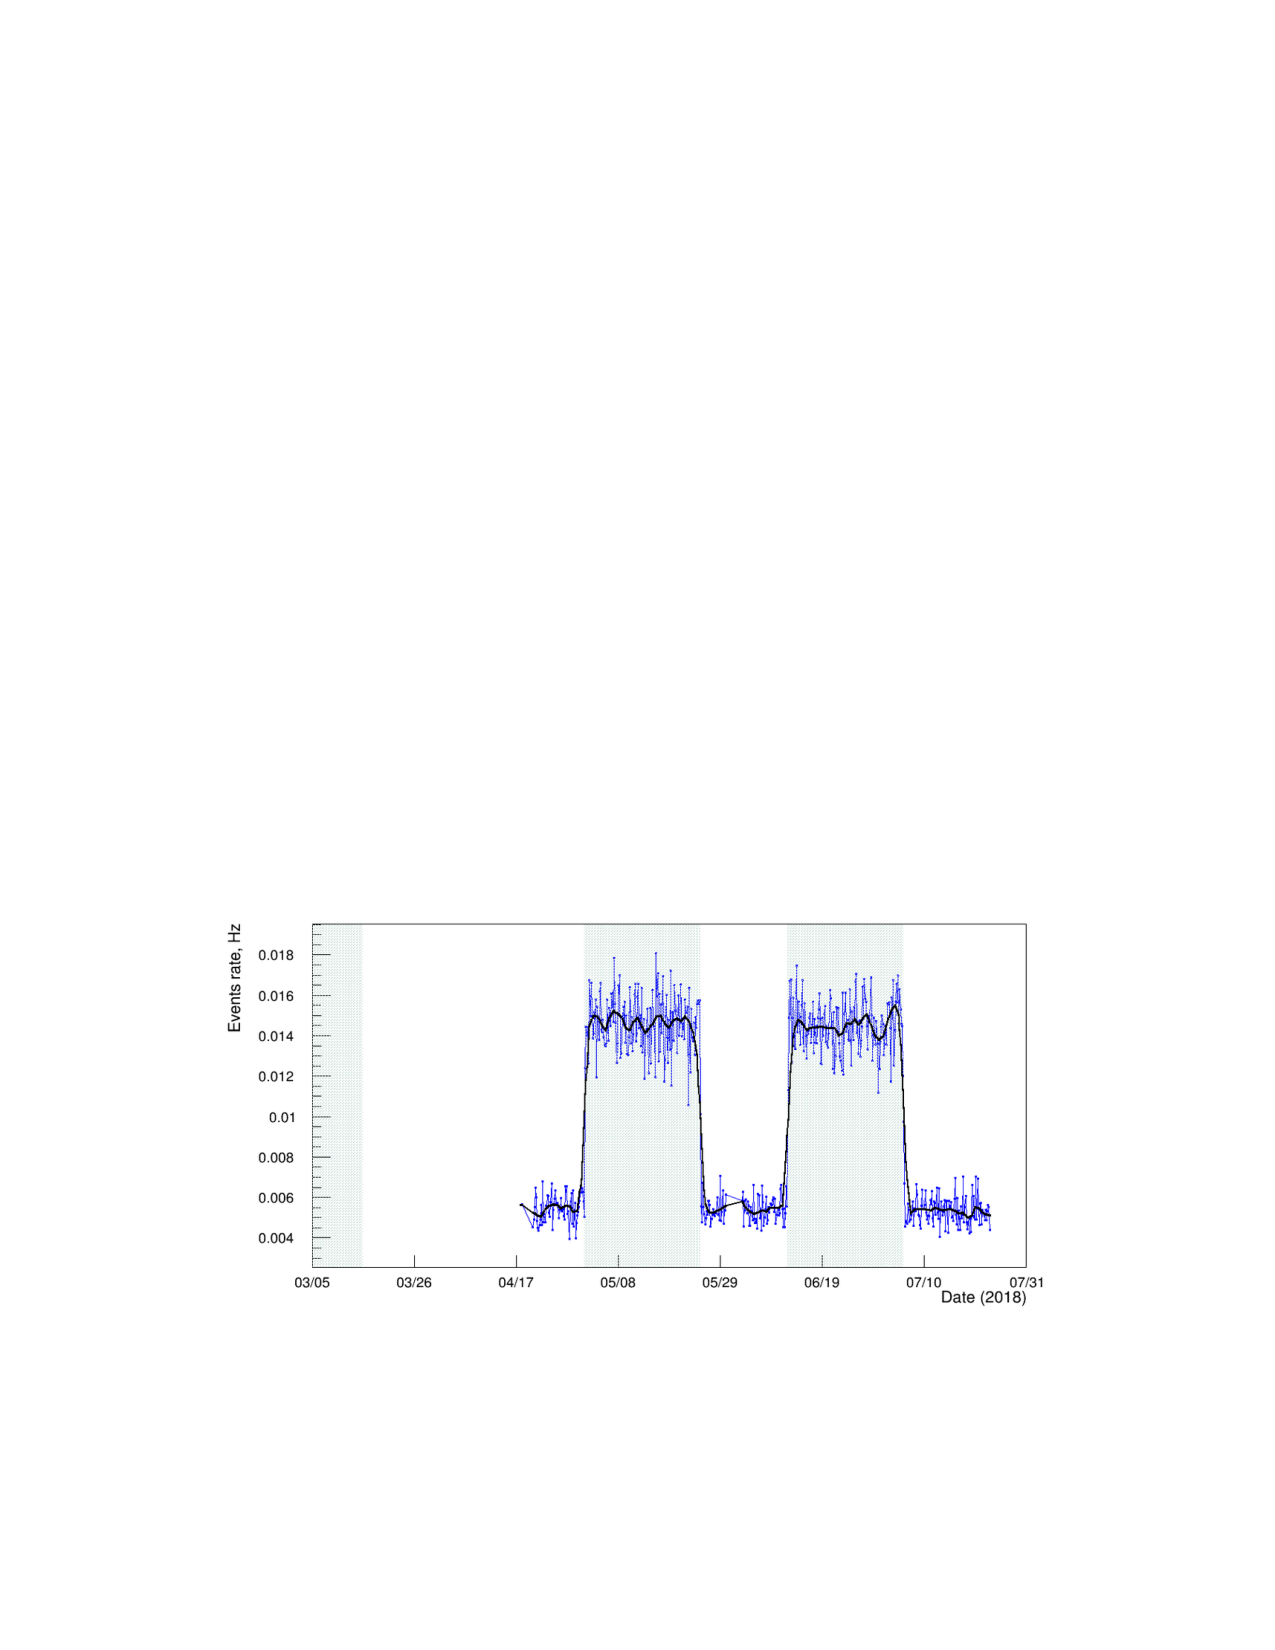
\includegraphics[width=0.85\textwidth]{Figures/IBDStability.pdf}
    \caption[IBD event rate stability]{
	The rate IBD correlated candidates with adjusted with local atmospheric pressure. 
	One data point is the event rate in every four hours.
    }
    \label{fig:IBDstability}
\end{figure}

The reactor-on and -off data dead time caused by the shower veto requirements varies from 14\% to 11\% of the total exposure time, due to reactor correlated time-varying gamma ray backgrounds that entered the nuclear recoil band.
Finally, a correction factor of 0.991$\pm$0.004 was multiplied to the background IBD prompt spectrum normalization by comparing the average reactor-on and -off atmospheric pressures~\cite{bib:ornl_weather} and dead time corrected exposure time.

The energy reconstruction stability of the IBD measurement was evaluated by comparing two reactor-off IBD prompt spectra equally divided, which is independent from possible power variation of the reactor.
The comparison between IBD prompt energy spectra from the two periods is shown in Figure~\ref{fig:BGstability}.
This two-period comparison validates the correction of atmospheric pressure, as well as the energy reconstruction stability, with $\chi^2/\mathrm{NDF} = 35.6/56$.

\begin{figure}[h!]
    \centering
    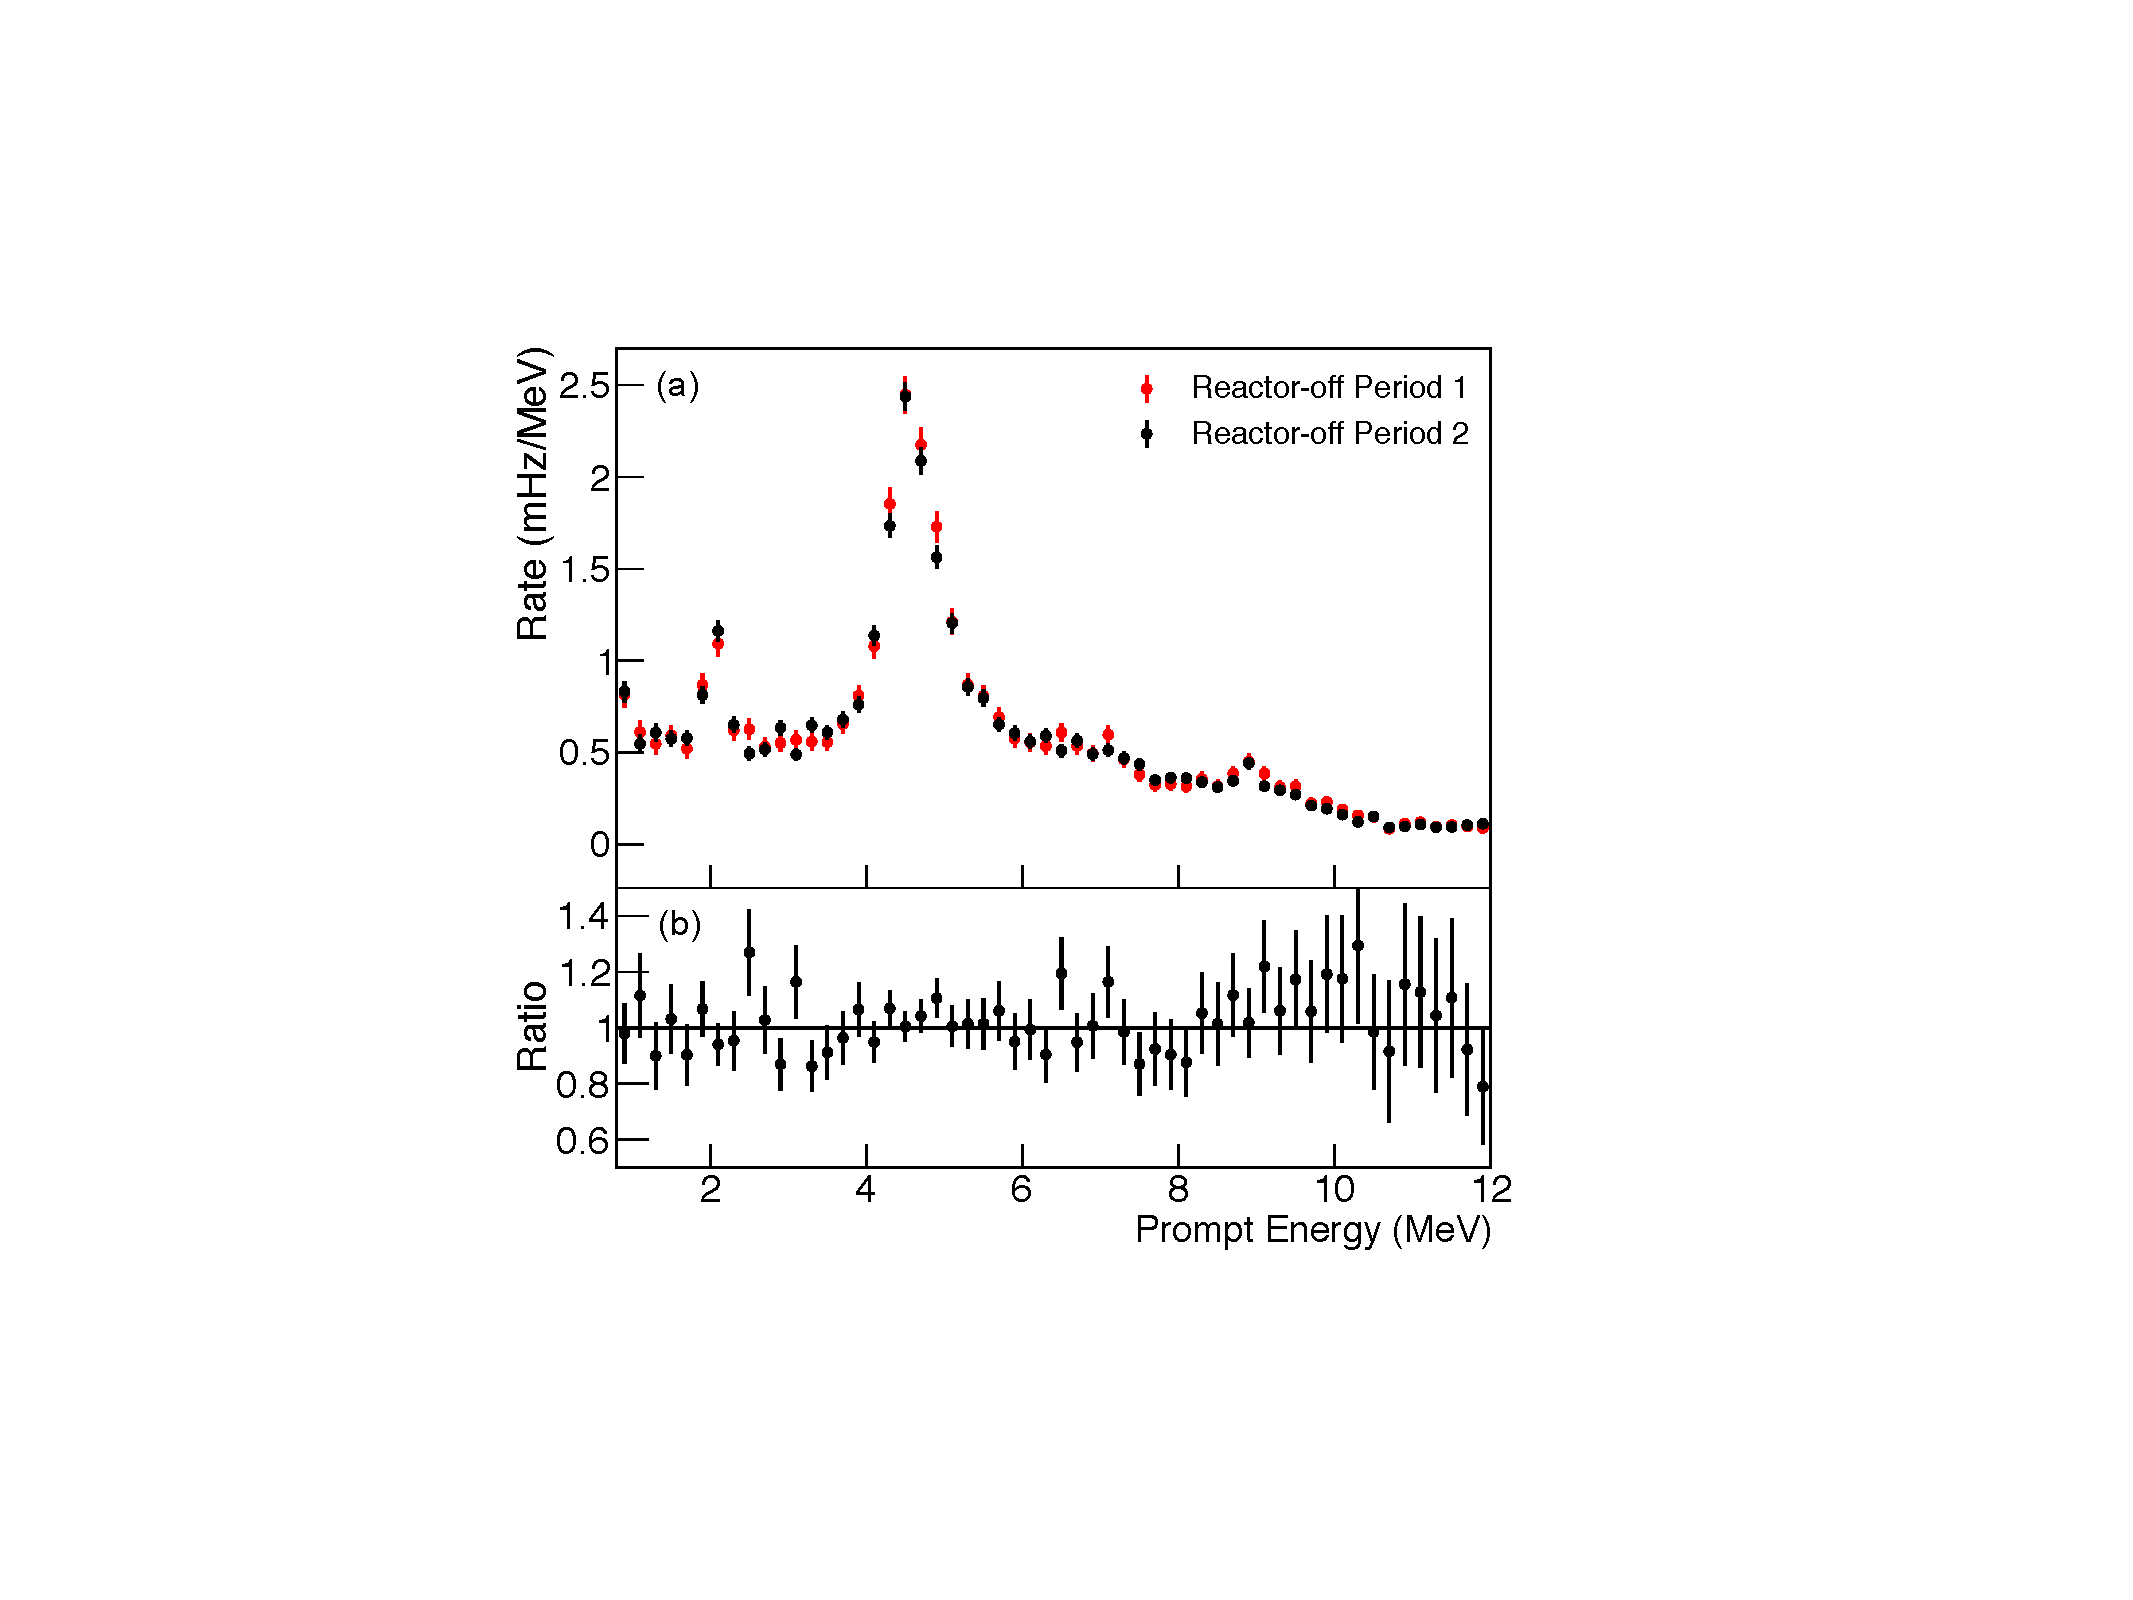
\includegraphics[width=0.8\textwidth]{Figures/BG_Stability.pdf}
    \caption[Reactor-off data energy stability]{
    The comparison between reactor-off energy spectra of two time periods. 
    (a) Energy spectra of reactor-off IBD candidate events with statistical errors. 
    (b) Ratio between two periods. }
    \label{fig:BGstability}
\end{figure}

\Section{IBD Prompt Energy Spectrum}

PROSPECT's first HFIR $^{235}$U reactor neutrino spectrum measurement included 40.3 exposure days of reactor-on data and 37.8 exposure days of reactor-off data.
In the energy range from 0.8~MeV to 7.2~MeV, total amount of reactor-on (-off) IBD candidates is 70811$\pm$267 (stat.) (20036$\pm$145 (stat.)) 
After subtraction of accidental events, there were 50277$\pm$267 (stat.) reactor-on correlated IBD candidates and 18600$\pm$145 (stat.) from reactor-off cycles.
The total number of reactor correlated IBD events is 31678$\pm$304 (stat.), with correlated S:B = 1.7:1.
The measured prompt energy spectrum is shown in Figure~\ref{fig:IBDspectrum}.
With 78~days of exposure, the IBD prompt energy spectrum of HFIR measured by PROSPECT became a direct $^{235}$U antineutrino spectrum measurement with the highest-ever precision, compared with $\sim$5000 IBD events measured in ILL~\cite{bib:ILL1985}.

\begin{figure}[h!]
    \centering
    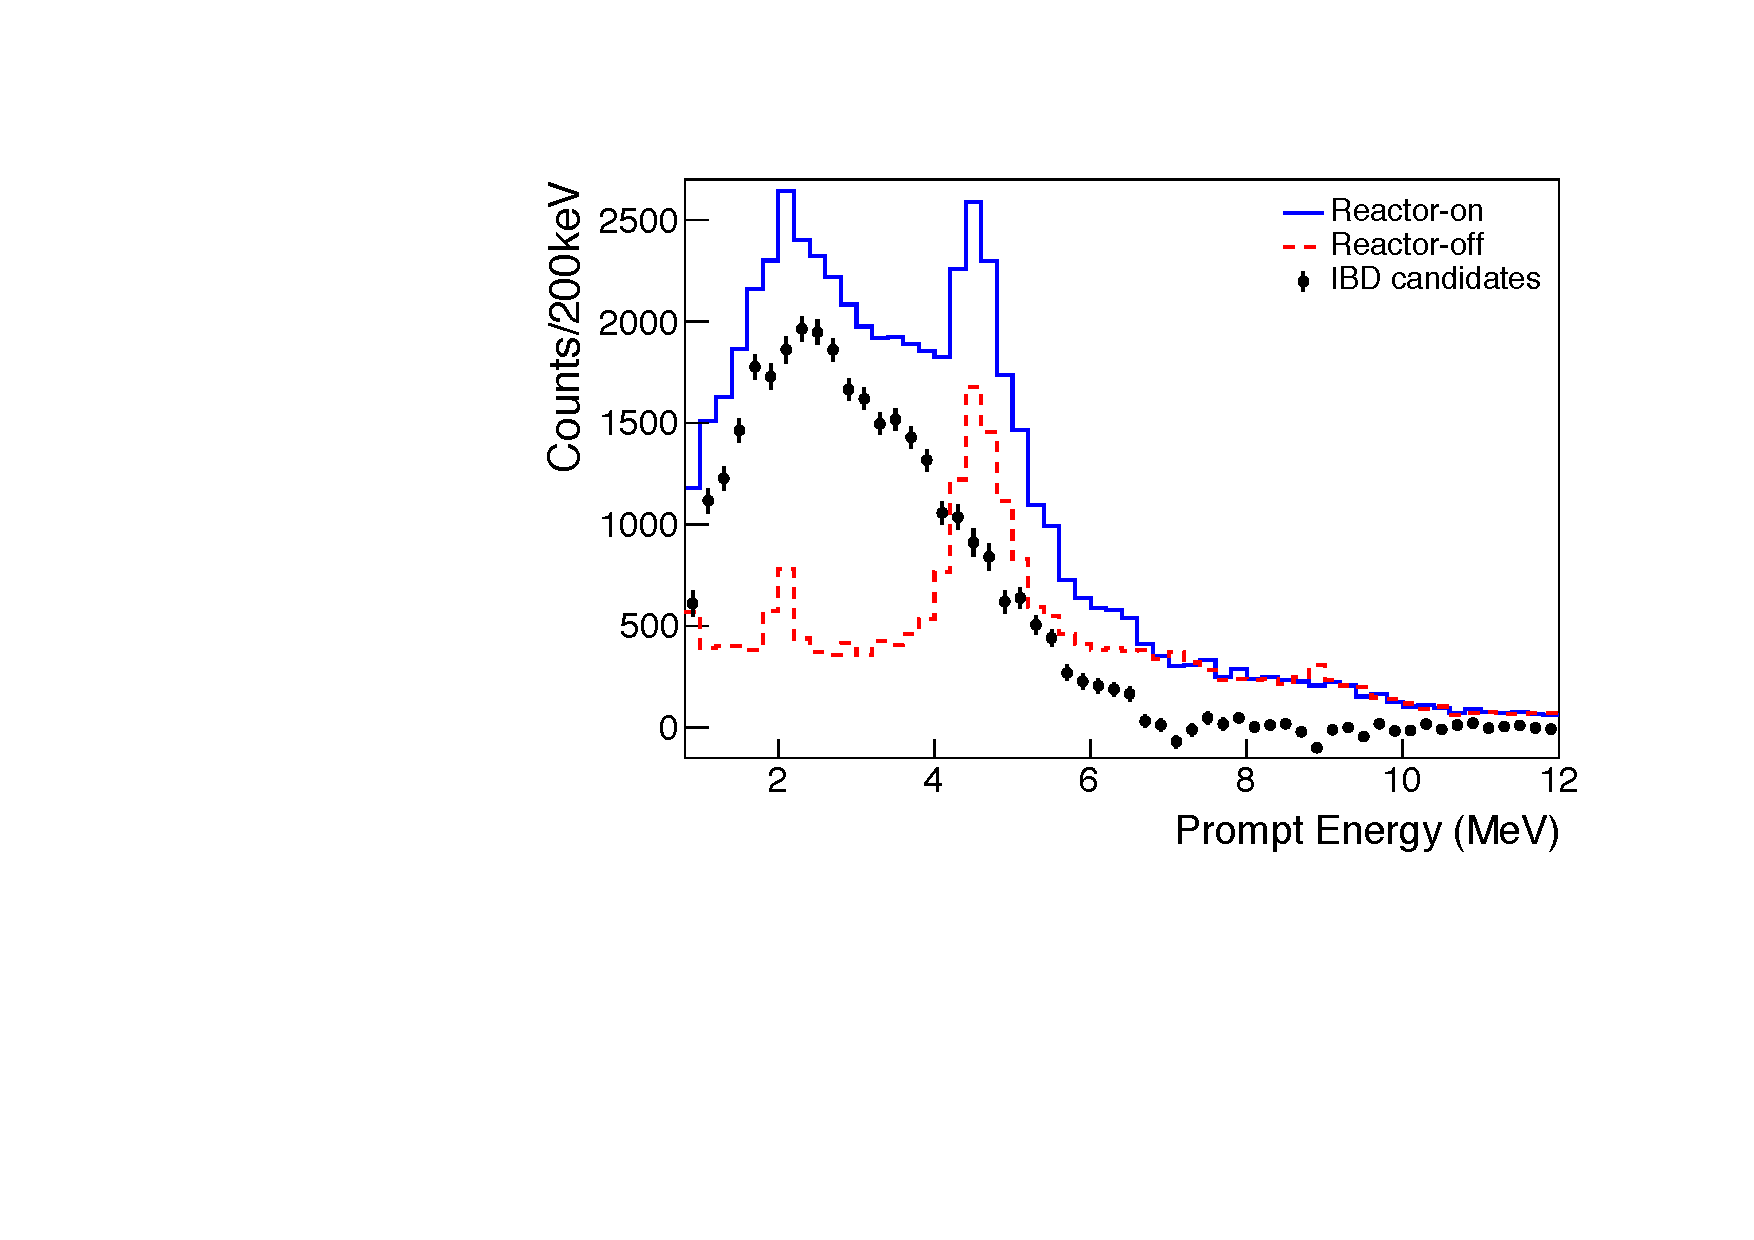
\includegraphics[width=0.75\textwidth]{Figures/h1IBDESpectrum.pdf}
    \caption[First PROSPECT IBD prompt energy spectrum from HFIR]{First PROSPECT IBD prompt energy spectrum from HFIR, where error bars indicates statistical error only.
    }
    \label{fig:IBDspectrum}
\end{figure}

\Section{Comparison with Spectrum Models}

The goal of the PROSPECT spectrum measurement is to test the $^{235}$U's contribution to previous LEU experiments' spectrum data-model disagreement, which is described in Chapter~\ref{Ch2}.
To achieve this goal, the IBD prompt energy spectrum of HFIR is subject to comparisons with spectrum models.
This study requires spectrum model generation, uncertainty processing, and hypothesis testing.

\Subsection{Spectrum Models}
Spectrum models were generated by multiplying a theoretical prediction of the neutrino spectrum with the IBD cross-section and the detector response matrix described in Section~\ref{sec:escalefinal}.
The multiplication with PROSPECT's detector response matrix maps antineutrino energy to PROSPECT reconstructed energy.
In this study, the Huber model of the $^{235}$U \nuebar spectrum~\cite{bib:huber} was compared to the PROSPECT measured spectrum under the assumption that no distortion of spectrum is caused by possible sterile neutrino oscillation.
In addition, two HFIR specific reactor correlated IBD sources were modeled as minor corrections to the models. 
The aluminum structure of the HFIR core generates \nuebar through $\beta$ decay of $^{28}$Al, whose half-life is 2.24~minutes and Q-value = 2.86~MeV. 
The short reactor cycle also introduces non-equilibrium fission isotopes that take days to achieve equilibrium of reaction.
Neutrinos from $^{28}$Al and non-equilibrium isotopes contributes to the IBD prompt spectrum mainly in the $<4$~MeV energy region, with $\sim$0.8\% and $\sim$0.5\% contribution factors, respectively.
The IBD prompt spectrum models with/without $^{28}$Al and non-equilibrium contribution are shown in Figure~\ref{fig:hubermodel}.
The contribution from spent nuclear fuel is negligible.
\begin{figure}[h!]
    \centering
    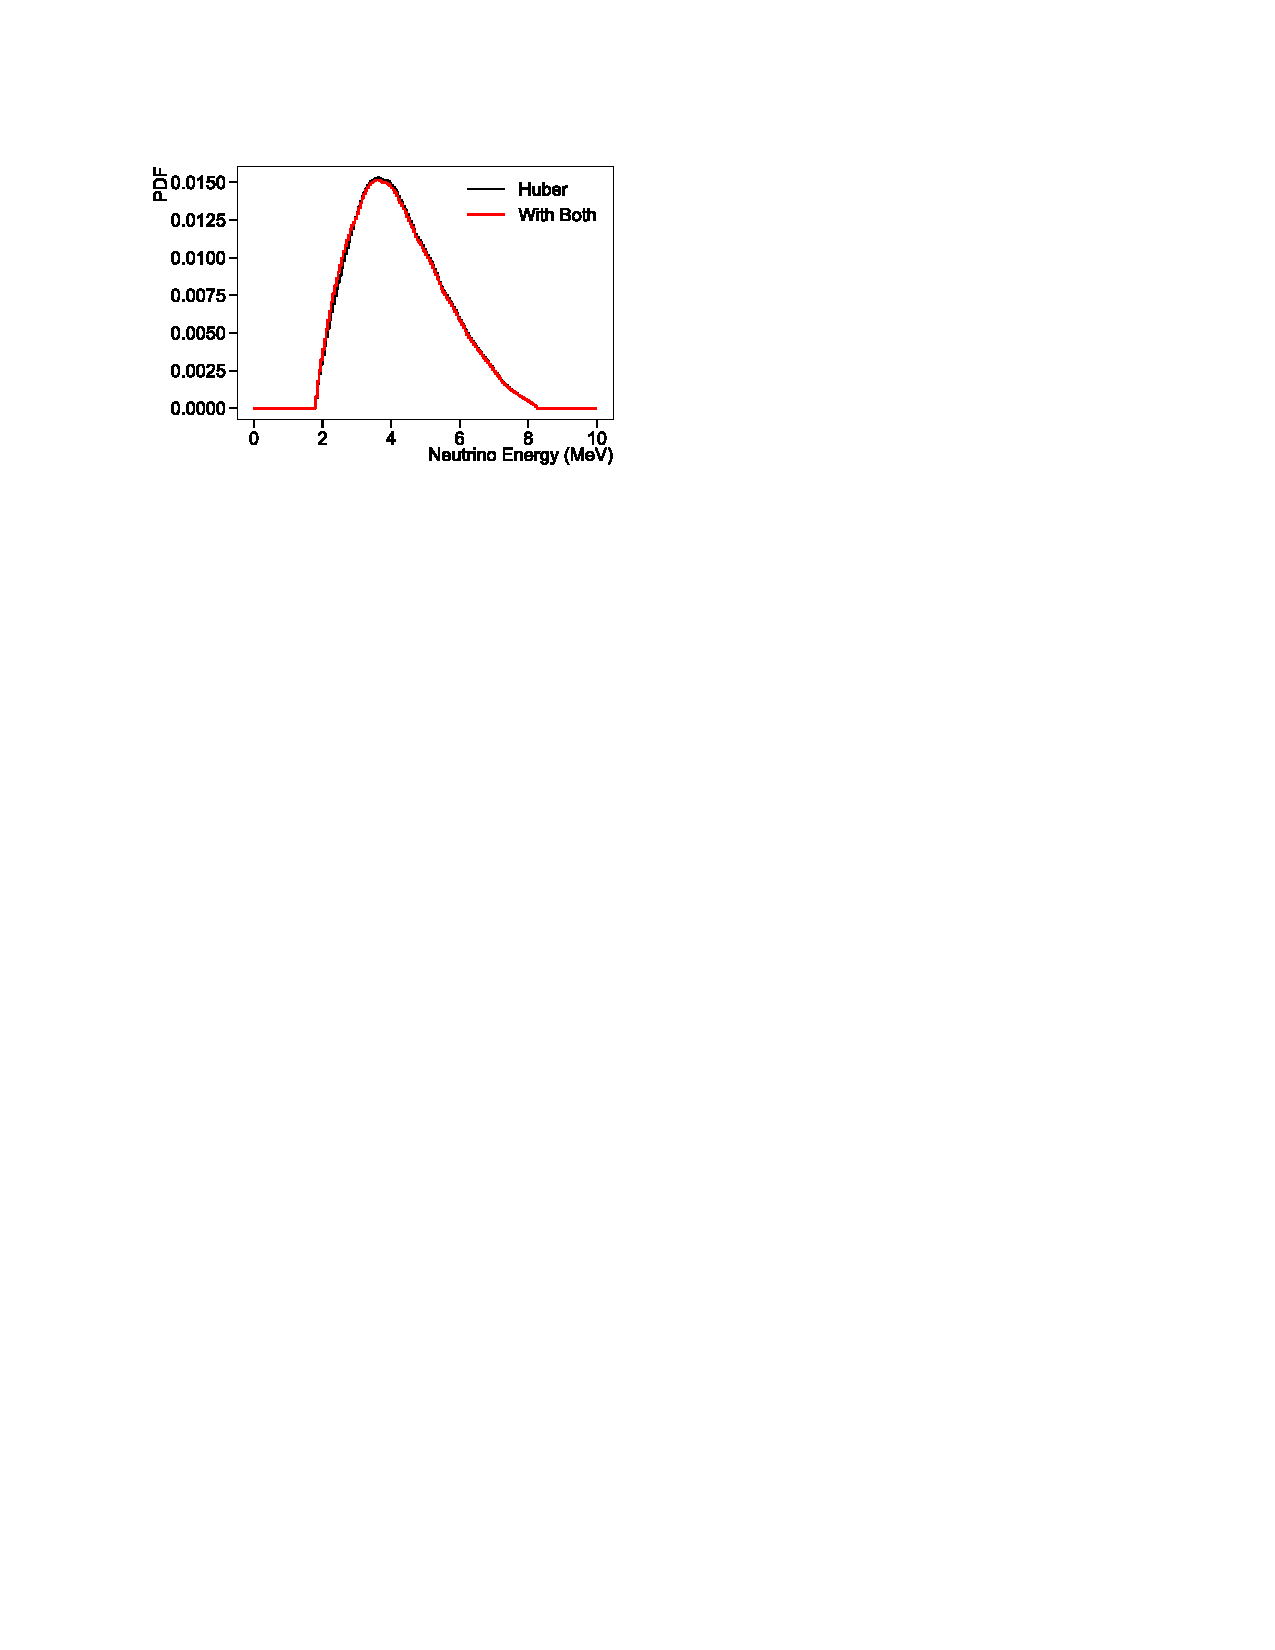
\includegraphics[width=0.6\textwidth]{Figures/HuberNoneq.pdf}
    \caption[Prompt spectrum model with Huber prediction]{
    Prompt spectrum model generated from Huber's prediction of $^{235}$U spectrum with the PG4 generated detector response matrix.
   	The spectrum model was adjusted with the contributions from $^{28}$Al decay and non-equilibrium isotopes in the HFIR core.}
    \label{fig:hubermodel}
\end{figure}

In order to search for the contribution of $^{235}$U to the spectral shape discrepancy observed in LEU neutrino experiments, the spectrum model was adjusted with a Gaussian function whose magnitude was allowed to float.

\Subsection{IBD Prompt Spectrum Data to Model Comparison}
Spectral shapes of the IBD data and model were compared through the evaluation of $\chi^2$,
\begin{equation}
\chi^2=  \mathbf{\Delta^{T}}  \mathbf{{V}^{-1}}  \mathbf{\Delta},  \\\nonumber 
\end{equation}
where
\begin{equation}
\Delta_i \equiv N_i^{obs} - N_i^{pred}\times (1 + \eta),
\label{eqn:min_chi2}
\end{equation}
where $\Delta_i$ is the difference between the experimental measurement and prediction, $\eta$ is a normalization nuisance parameter and $\mathbf{V}$ is a full covariance matrix, processing statistical and systematic uncertainties.  
This full covariance matrix was summed from covariance matrices of uncertainties of various aspects of analysis, such as the energy model uncertainty described in Section~\ref{sec:escalefinal}.
A single covariance matrix was produced by comparing IBD spectrum models to toy spectra with specific variables allowed to vary within a predetermined uncertainty range.
The systematic uncertainties studied and included in the covariance matrix are listed in Table~\ref{tab:Covs}.
The full covariance matrix for data for the model comparison is shown in Figure~\ref{fig:covs}.

   \begin{longtable}{p{3cm}p{2cm}p{8cm}}
    %\centering
   	\caption[List of systematic uncertainties]{List of systematic uncertainties.}\\
     \hline 
     \hline 
     Systematic uncertainty & $\sigma$ & Description \\ 
     \hline
     Background normalization & 0.5\% & uncertainty of the time dependent event rate  \\ 
     Background $n$-H peak height & 4\% & the variation of $n$-H peak height \\
     \hline
     Energy reconstruction factors &  - & described in detail Section~\ref{sec:escalefinal}\\
     Energy leakage & 8~keV & the data to MC difference of in energy shift from $^{22}$Na calibration at different positions in detector\\
     \hline
     $z$ fiducial volume & 25~mm & position reconstruction variation\\
     $^{28}$Al contribution & 100\% & uncertainty of contribution factor to the spectrum\\
	Non-equilibrium isotope contribution & 100\% & uncertainty of contribution factor to the spectrum\\
     \hline
     \label{tab:Covs}   
   \end{longtable}
   
\begin{figure}[h!]
    \centering
    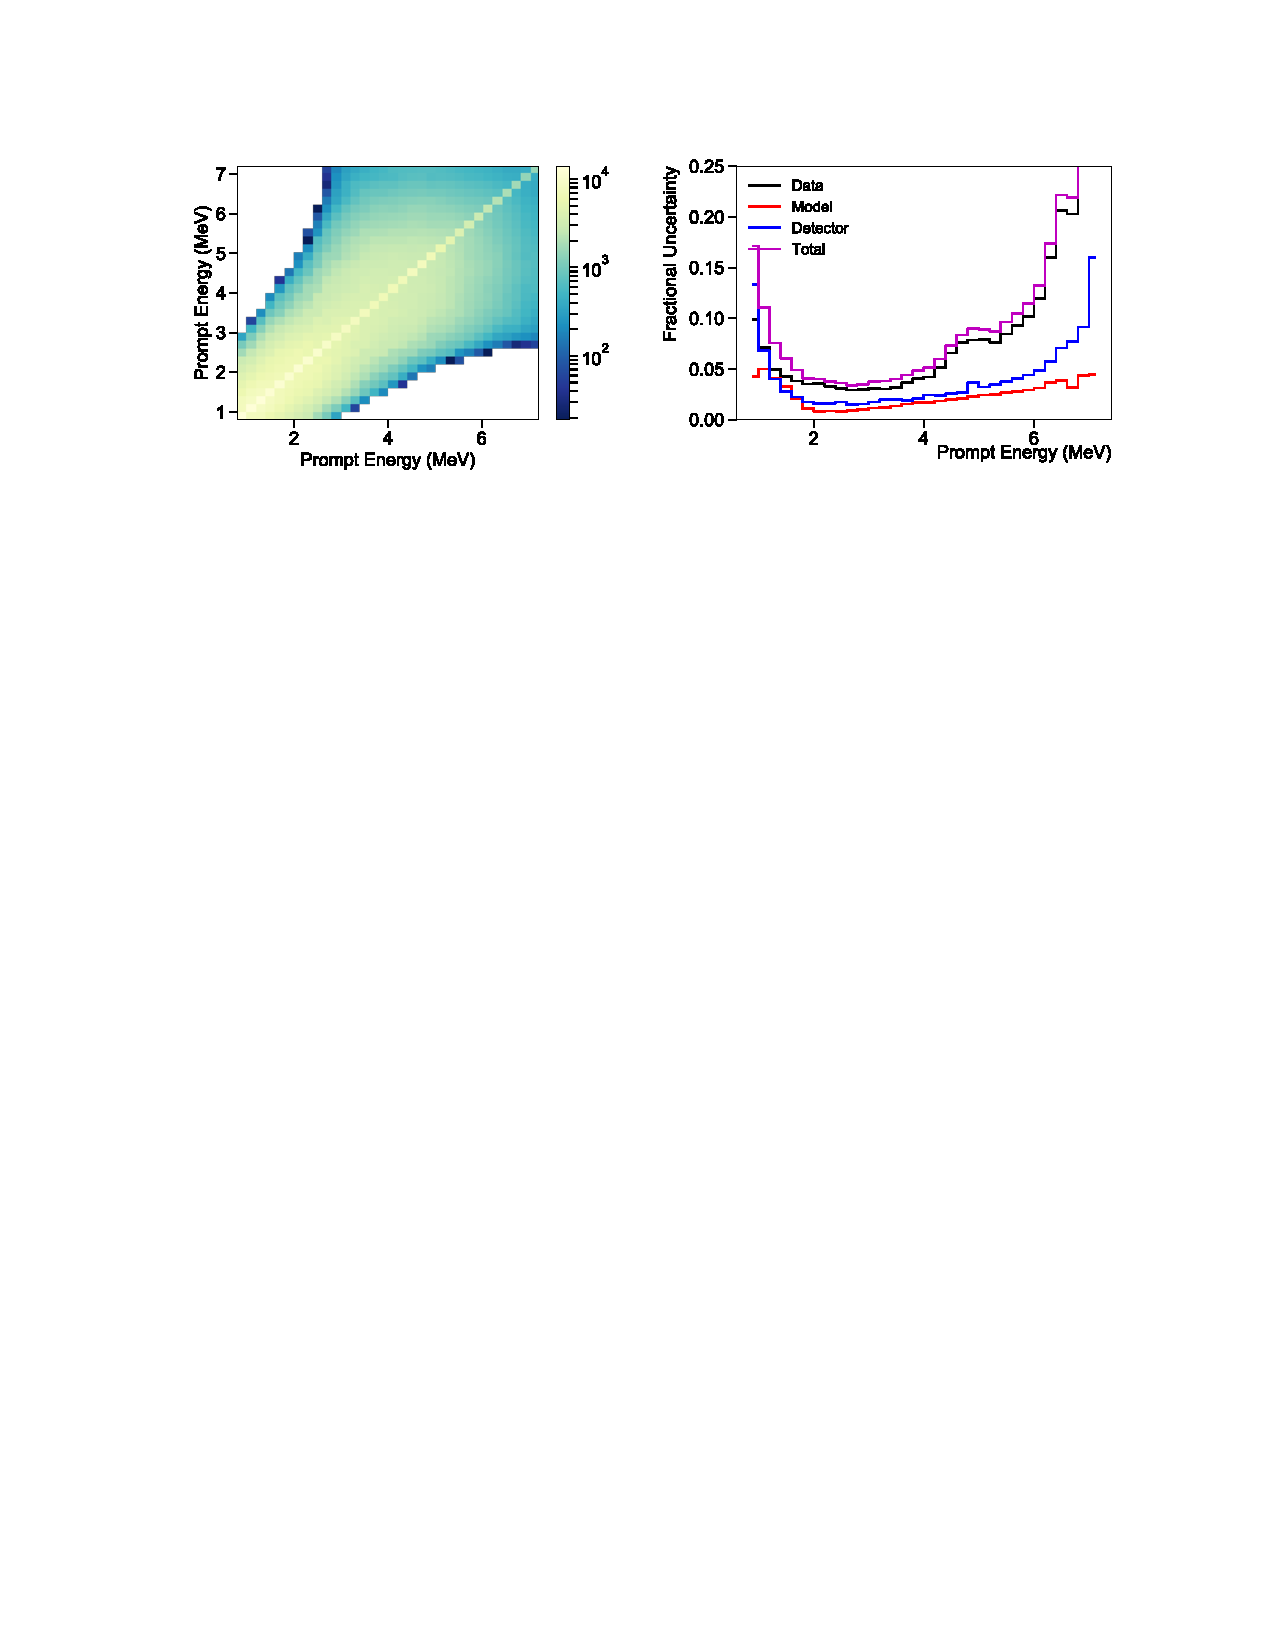
\includegraphics[width=0.98\textwidth]{Figures/CovMatrix.pdf}
    \caption[Full covariance matrix for the PROSPECT spectrum analysis]{
    (Left) Full covariance matrix used in PROSPECT spectrum and model comparison.
    (Right) The diagonal terms of the different covariance matrices.
   	Currently, the uncertainty of PROSPECT's spectrum measurement is statistically dominated.}
    \label{fig:covs}
\end{figure}

The spectral shape contribution to the total $\chi^2$ in different energy range is defined as 
\begin{equation}
\widetilde{\chi_i} = \frac{N_i^{obs}-N_i^{pred}}{|N_i^{obs}-N_i^{pred}|} \sqrt{\chi^2_{original} - \chi^2_{i,new}}.
\end{equation}
The energy distribution of the local $\chi^2_i$ is used to characterize the deviation in each energy bin.
The PROSPECT measured IBD prompt spectrum is shown in Figure~\ref{fig:modelcompare}, along with local $\chi^2$ contributions and data-model ratios.

\begin{figure}[h!]
    \centering
    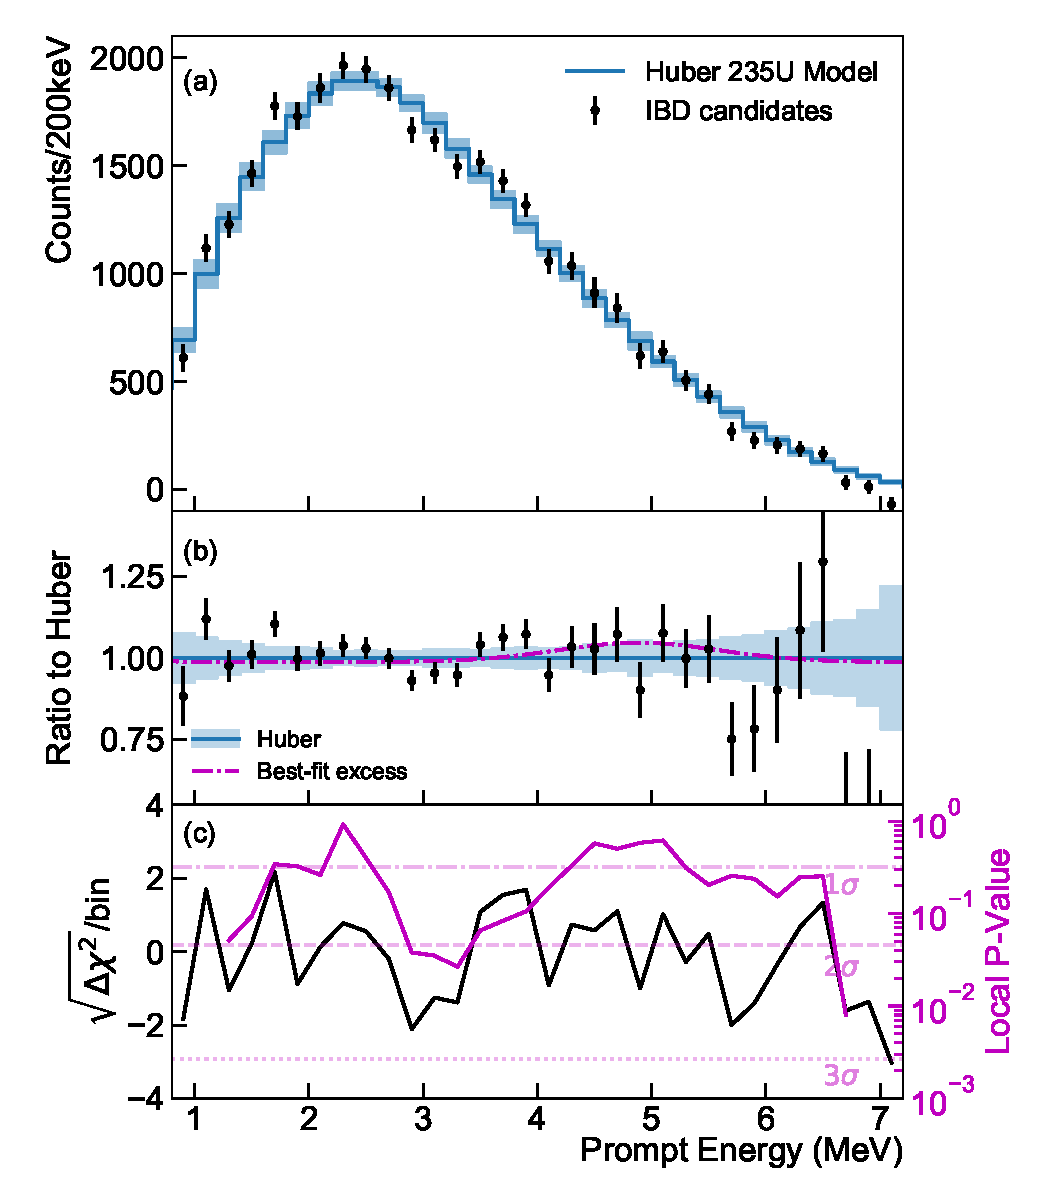
\includegraphics[width=0.7\textwidth]{Figures/CombinedComparison.pdf}
    \caption[PROSPECT measured spectrum compared to adjusted Huber spectral model]{
    (a) PROSPECT measured spectrum compared to adjusted Huber spectral model~\cite{bib:prospect_spec}, with error bars including both statistical and systematic uncertainties.
    (b) The IBD prompt spectrum ratio to the adjusted Huber model, a best-fit \textit{ad hoc} distortion to the model at the 4-6~MeV region.
    (c) The $\chi^2$ constribution from each energy bin and the local $p$-values in 1~MeV wide regions.}
    \label{fig:modelcompare}
\end{figure}

\Subsection{Results}
In the comparison between the PROSPECT measured spectrum and the  adjusted Huber spectrum model, $\chi^2/\mathrm{NDF} = 51.4/31$, with a one-sided $p = 0.01$.
Most significant local discrepancies were found in the range from 2.8~MeV to 3.5~MeV, and $>$ 6.5~MeV energy, with $2-3\sigma$ significance.

An \textit{ad hoc} spectrum model was made based on the Huber spectrum to allow regional spectral shape, in 5-7~MeV \nuebar energy, to change with a Gaussian.
The best-fit \textit{ad hoc} spectrum model is shown in Figure~\ref{fig:modelcompare}(b), suggesting a distortion magnitude $n = 0.69\pm0.53$ observed by PROSPECT, as a ratio to Daya Bay measured magnitude of excess~\cite{bib:DYBSpectrum}.
This result is compatible with hypothesis of equal isotopic contribution ($n = 1$) and the Huber model ($n = 0$), with current uncertainties.
The PROSPECT measured IBD spectrum disfavors (with $2.1\sigma$) the hypothesis that the regional excess is caused solely from $^{235}$U ( $n = 1.78$). 


